\documentclass[12pt,a4paper]{article}
\usepackage[utf8]{inputenc}\usepackage[T1]{fontenc}\usepackage[brazil]{babel}\usepackage{lmodern}
\usepackage{geometry}\geometry{margin=2.3cm}
\usepackage{graphicx}\graphicspath{{figuras/}}
\usepackage{booktabs,tabularx,array,multirow,amsmath,amssymb,siunitx,xcolor,float}
\sisetup{output-decimal-marker={,}}
\usepackage[section]{placeins}\usepackage{enumitem,microtype,caption,subcaption,listings,hyperref,fancyhdr}
\hypersetup{colorlinks=true,linkcolor=blue!55!black,urlcolor=blue!55!black,citecolor=blue!55!black}
\lstdefinestyle{sindyeq}{basicstyle=\ttfamily\scriptsize,breaklines=true,breakatwhitespace=false,columns=fullflexible,frame=single,numbers=left,numberstyle=\tiny\color{gray},xleftmargin=1.5em,framexleftmargin=1.2em,showstringspaces=false}
\pagestyle{fancy}\fancyhf{}\lhead{Dam-break URANS e modelos reduzidos}\rhead{Relatório técnico}\cfoot{\thepage}
\setlength{\parindent}{1.2em}\setlength{\parskip}{0.35em}
\newcommand{\code}[1]{\texttt{#1}}
\title{\textbf{Relatório técnico do caso dam-break URANS}\\[0.4em]OpenFOAM, POD, SAE e identificação dinâmica SINDy}
\author{Análise dos códigos e resultados armazenados no caso}\date{\today}
\begin{document}\maketitle
\begin{abstract}
Documenta-se o caso dam-break bifásico calculado no OpenFOAM 13 com URANS $k$--$\omega$ SST, as reduções POD e SAE e três modelos SINDy: POD--SINDy, SAE--SINDy e SAE--POD--SINDy. Os parâmetros e métricas foram extraídos dos dicionários, modelos Keras, NPZ, JSON e CSV efetivamente salvos. A POD com 50 modos preserva 99,36\% da energia da velocidade e apresenta erro global de 8,02\%. O SAE salvo reconstrói cinco campos com $R^2$ próximo de 0,95. Entretanto, POD--SINDy e SAE--SINDy falham na integração livre e seus baixos erros guiados medem apenas fidelidade local. A POD equidimensional aplicada aos quatro latentes preserva praticamente 100\% da energia, permite integração livre e produz $R^2=0,697$ na trajetória reduzida, resultado coerente com o papel estabilizador discutido por Lin, Xiao e Fang. Ainda assim, o erro relativo livre de 0,551 mostra que o modelo não é uma reprodução dinâmica exata.
\end{abstract}
\tableofcontents\listoffigures\listoftables\clearpage

\section{Escopo e rastreabilidade}
O caso analisado está em
\begin{quote}\small\path{/home/mlep-pc-ubuntu/OpenFOAM/mlep-pc-ubuntu-13/run/damBreakLaminar(URANS)10.000}.\end{quote}
Foram usados os dicionários OpenFOAM, os notebooks em \code{POD/src}, \code{SAE/src} e \code{SINDy/src}, e os artefatos em \code{resultados}. Os cálculos não foram refeitos.

Há divergências entre o notebook SAE atual e os artefatos: o notebook declara grade $48\times48$ e oito latentes, enquanto o modelo Keras salvo tem entrada 5120, equivalente a $32\times32\times5$, e quatro latentes. O NPZ também contém quatro latentes. Os tempos de treino e validação estão distribuídos por quase todo o intervalo, embora a função atualmente escrita no notebook faça divisão temporal. Consequentemente, os resultados são descritos a partir dos artefatos, e a configuração textual divergente é tratada como versão não sincronizada. A POD salva possui dimensão 4536, isto é, somente $U_x,U_y$ em 2268 células, apesar de o notebook atual listar campos adicionais.

\section{Simulação OpenFOAM URANS}
\subsection{Problema físico, malha e propriedades}
O solver é \code{incompressibleVoF}, com água e ar, gravidade $(0,-9{,}81,0)\,\si{m.s^{-2}}$ e tensão superficial \SI{0.07}{N.m^{-1}}. A coluna inicial ocupa $0\le x\le\SI{0.1461}{m}$ e $0\le y\le\SI{0.292}{m}$. O domínio nominal é $0{,}584\times0{,}584\times0{,}0146\,\si{m^3}$. Os cinco blocos têm 2268 células e apenas uma célula em $z$, com faces correspondentes do tipo \code{empty}; trata-se de aproximação quase bidimensional.

\begin{table}[H]\centering
\caption{Modelo físico e de turbulência URANS.}\label{tab:fisica}
\begin{tabularx}{\textwidth}{>{\bfseries}l X}
\toprule Item & Configuração\\\midrule
Solver & \code{incompressibleVoF}, OpenFOAM 13\\
Água & $\rho=1000\,\si{kg.m^{-3}}$, $\nu=10^{-6}\,\si{m^2.s^{-1}}$\\
Ar & $\rho=1\,\si{kg.m^{-3}}$, $\nu=1{,}48\times10^{-5}\,\si{m^2.s^{-1}}$\\
Turbulência & \code{simulationType RAS}, modelo $k$--$\omega$ SST\\
Malha & 2268 células, cinco blocos, uma célula em $z$\\
Contornos & paredes esquerda/direita/inferior; atmosfera no topo\\
\bottomrule\end{tabularx}\end{table}
Embora a pasta contenha ``Laminar'', o dicionário ativa RAS $k$--$\omega$ SST; a classificação correta é URANS.

\subsection{Discretização e solução algébrica}
\begin{table}[H]\centering
\caption{Discretização OpenFOAM.}\label{tab:disc}
\begin{tabularx}{\textwidth}{>{\bfseries}l X}
\toprule Item & Configuração\\\midrule
Tempo & Euler de primeira ordem; $\Delta t=10^{-4}\,\si{s}$ fixo; $0\le t\le1\,\si{s}$\\
Saída & todo passo: 10001 diretórios, incluindo os extremos\\
Gradientes & Gauss linear; esquema \code{limitedGrad} para turbulência\\
VOF & \code{interfaceCompression vanLeer 1}\\
Momento & Gauss \code{linearUpwind grad(U)}\\
$k,\omega$ & Gauss \code{linearUpwind limitedGrad}\\
Laplaciano/$\mathrm{snGrad}$ & linear uncorrected / uncorrected\\
Passo adaptativo & desativado; $Co$ configurado em 1, mas sem controle adaptativo\\
\bottomrule\end{tabularx}\end{table}

\begin{table}[H]\centering
\caption{Solvers e acoplamento.}\label{tab:solvers}
\begin{tabularx}{\textwidth}{>{\bfseries}l X}
\toprule Bloco & Configuração\\\midrule
$\alpha_{water}$ & 2 corretores, 1 subciclo; MULES 10 iterações, tolerância $10^{-2}$; solver tolerância $10^{-8}$\\
$p_{rgh}$ & PCG/DIC, tolerância $10^{-7}$, \code{relTol}=0,05; final com zero\\
$U,k,\omega$ & \code{smoothSolver}/\code{symGaussSeidel}, tolerância $10^{-6}$\\
PIMPLE & 1 corretor externo, 3 internos, 0 não ortogonais; preditor de momento desligado\\
\bottomrule\end{tabularx}\end{table}

Os pontos positivos são o passo pequeno e os 10001 snapshots. Como limitações, Euler é dissipativo e de primeira ordem, não há controle adaptativo efetivo de Courant, a malha tem uma célula em $z$ e não foi localizado estudo de convergência ou validação experimental.

\section{POD da velocidade}
Os artefatos armazenam $X\in\mathbb{R}^{4536\times10001}$, formado por $U_x,U_y$ nas 2268 células. Cada snapshot foi normalizado, os dados foram centralizados e decompostos por
\begin{equation}X-\overline X=U\Sigma V^T,\qquad X_r=U_r\Sigma_rV_r^T.\end{equation}
Foram avaliados 1 a 50 modos; 10\% dos instantes foram separados aleatoriamente para diagnóstico de teste.

\begin{table}[H]\centering
\caption{Energia e erro POD.}\label{tab:pod}
\begin{tabular}{rcc}\toprule Modos & Energia acumulada & Erro global\\\midrule
1&0,4189&0,7623\\2&0,5748&0,6521\\4&0,7284&0,5212\\8&0,8462&0,3922\\16&0,9335&0,2580\\32&0,9803&0,1405\\50&0,9936&0,0802\\\bottomrule\end{tabular}\end{table}

\begin{figure}[H]\centering
\begin{subfigure}{.49\textwidth}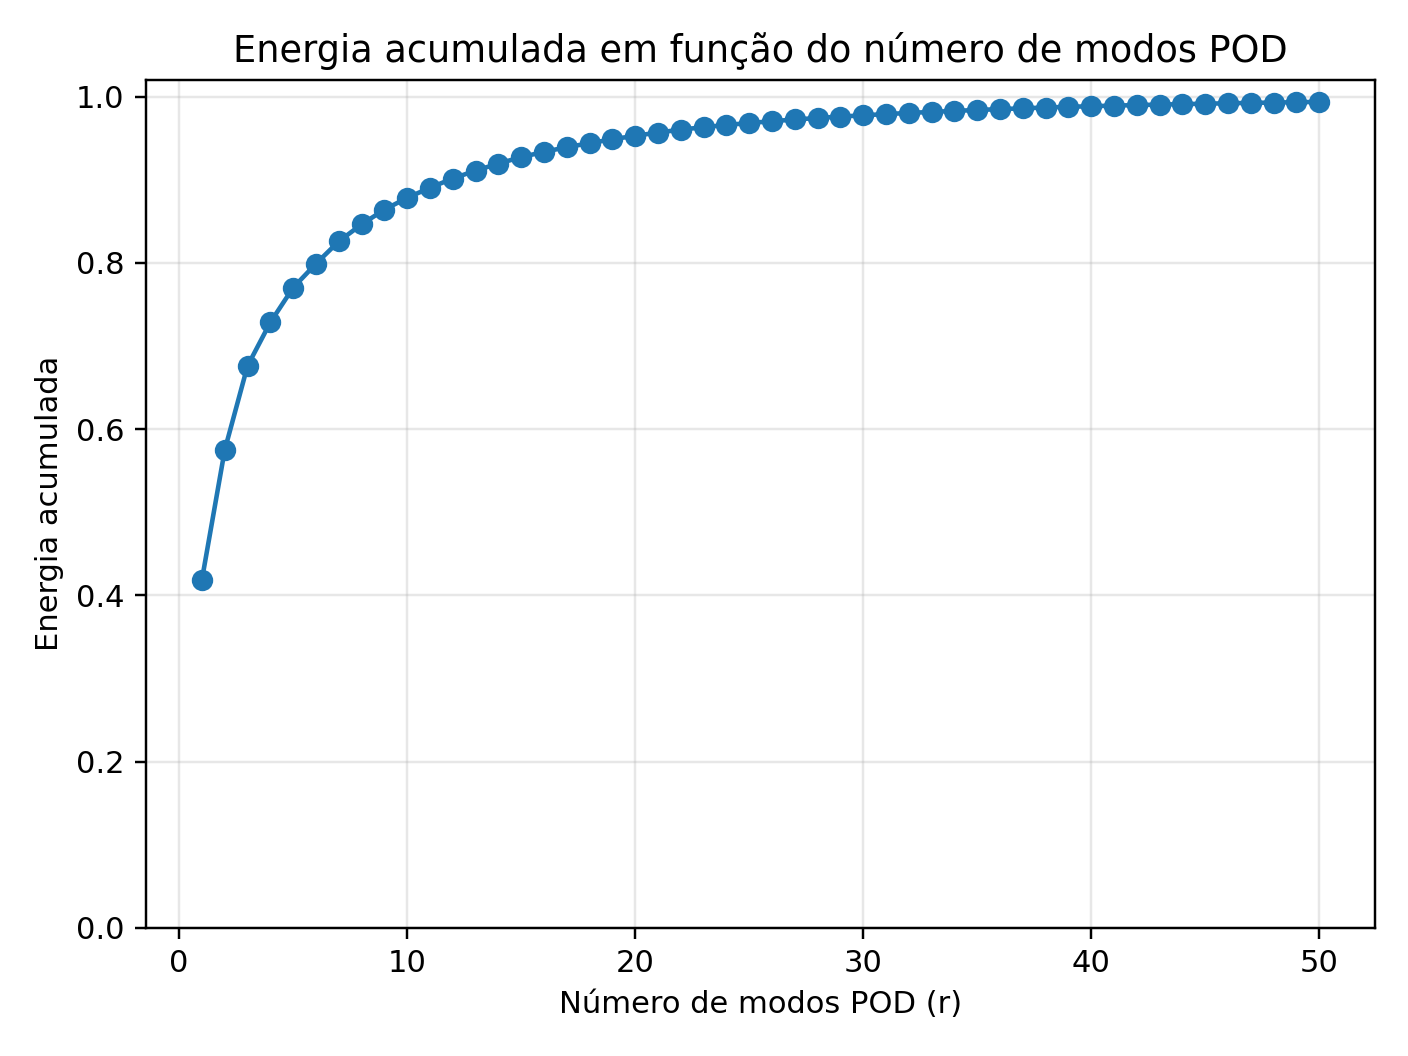
\includegraphics[width=\linewidth]{pod_energia.png}\caption{Energia.}\end{subfigure}
\begin{subfigure}{.49\textwidth}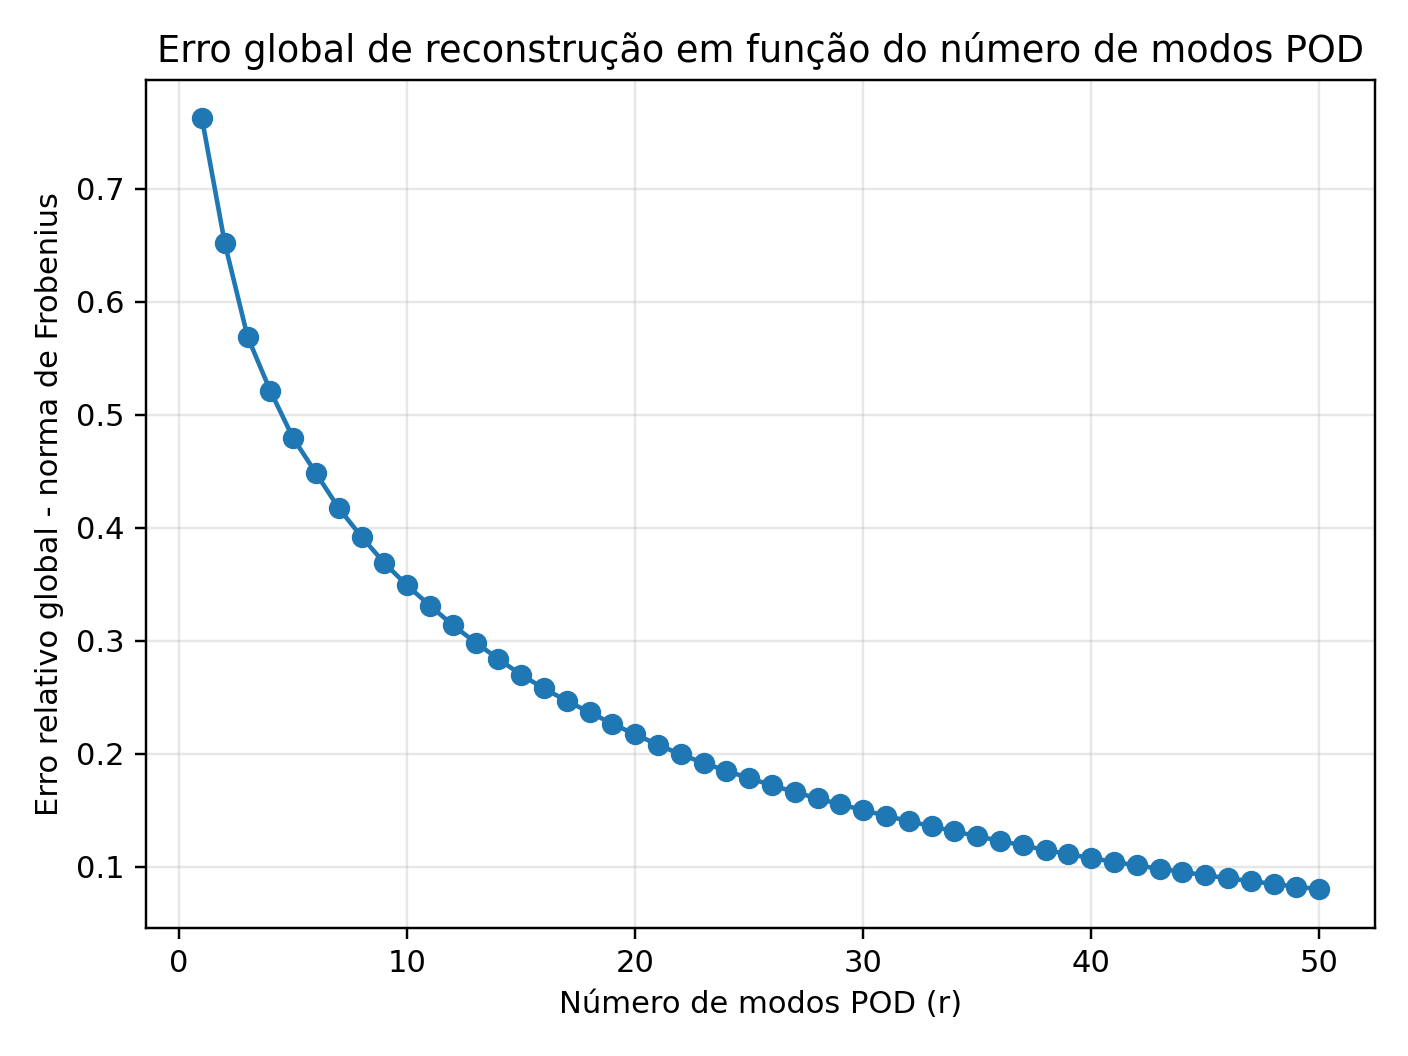
\includegraphics[width=\linewidth]{pod_erro.png}\caption{Erro global.}\end{subfigure}
\caption{Convergência da POD da velocidade.}\end{figure}
\begin{figure}[H]\centering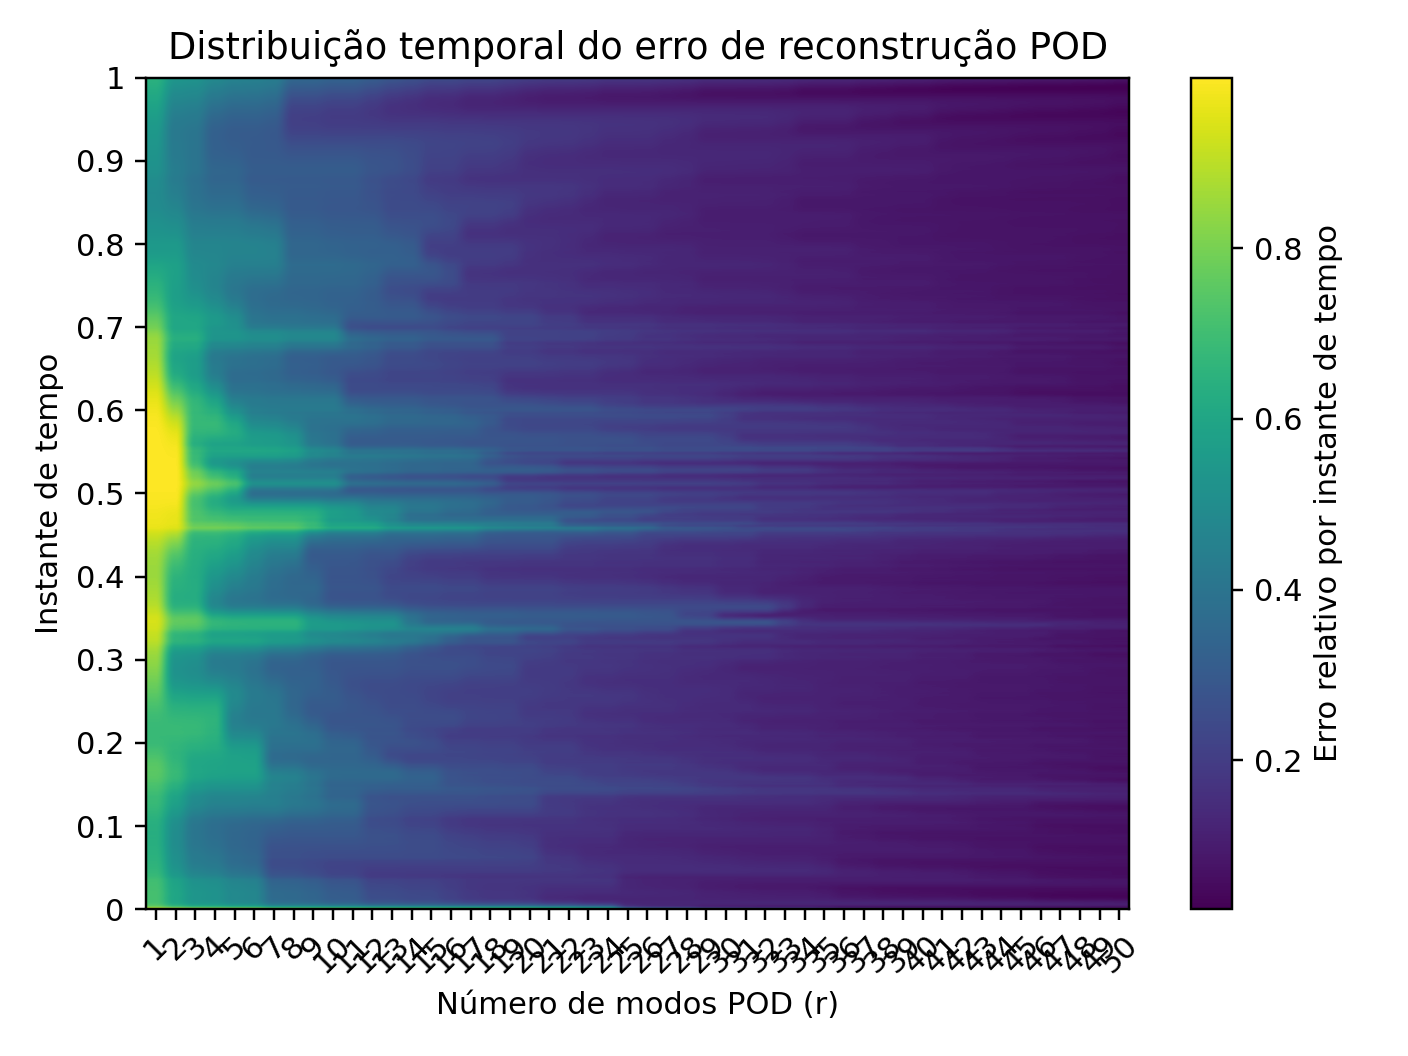
\includegraphics[width=.9\textwidth]{pod_mapa.png}\caption{Erro temporal em função do número de modos. O maior erro com 50 modos é 0,763 e ocorre no início, quando a velocidade tem norma quase nula e o erro relativo se torna mal condicionado.}\end{figure}
\begin{figure}[H]\centering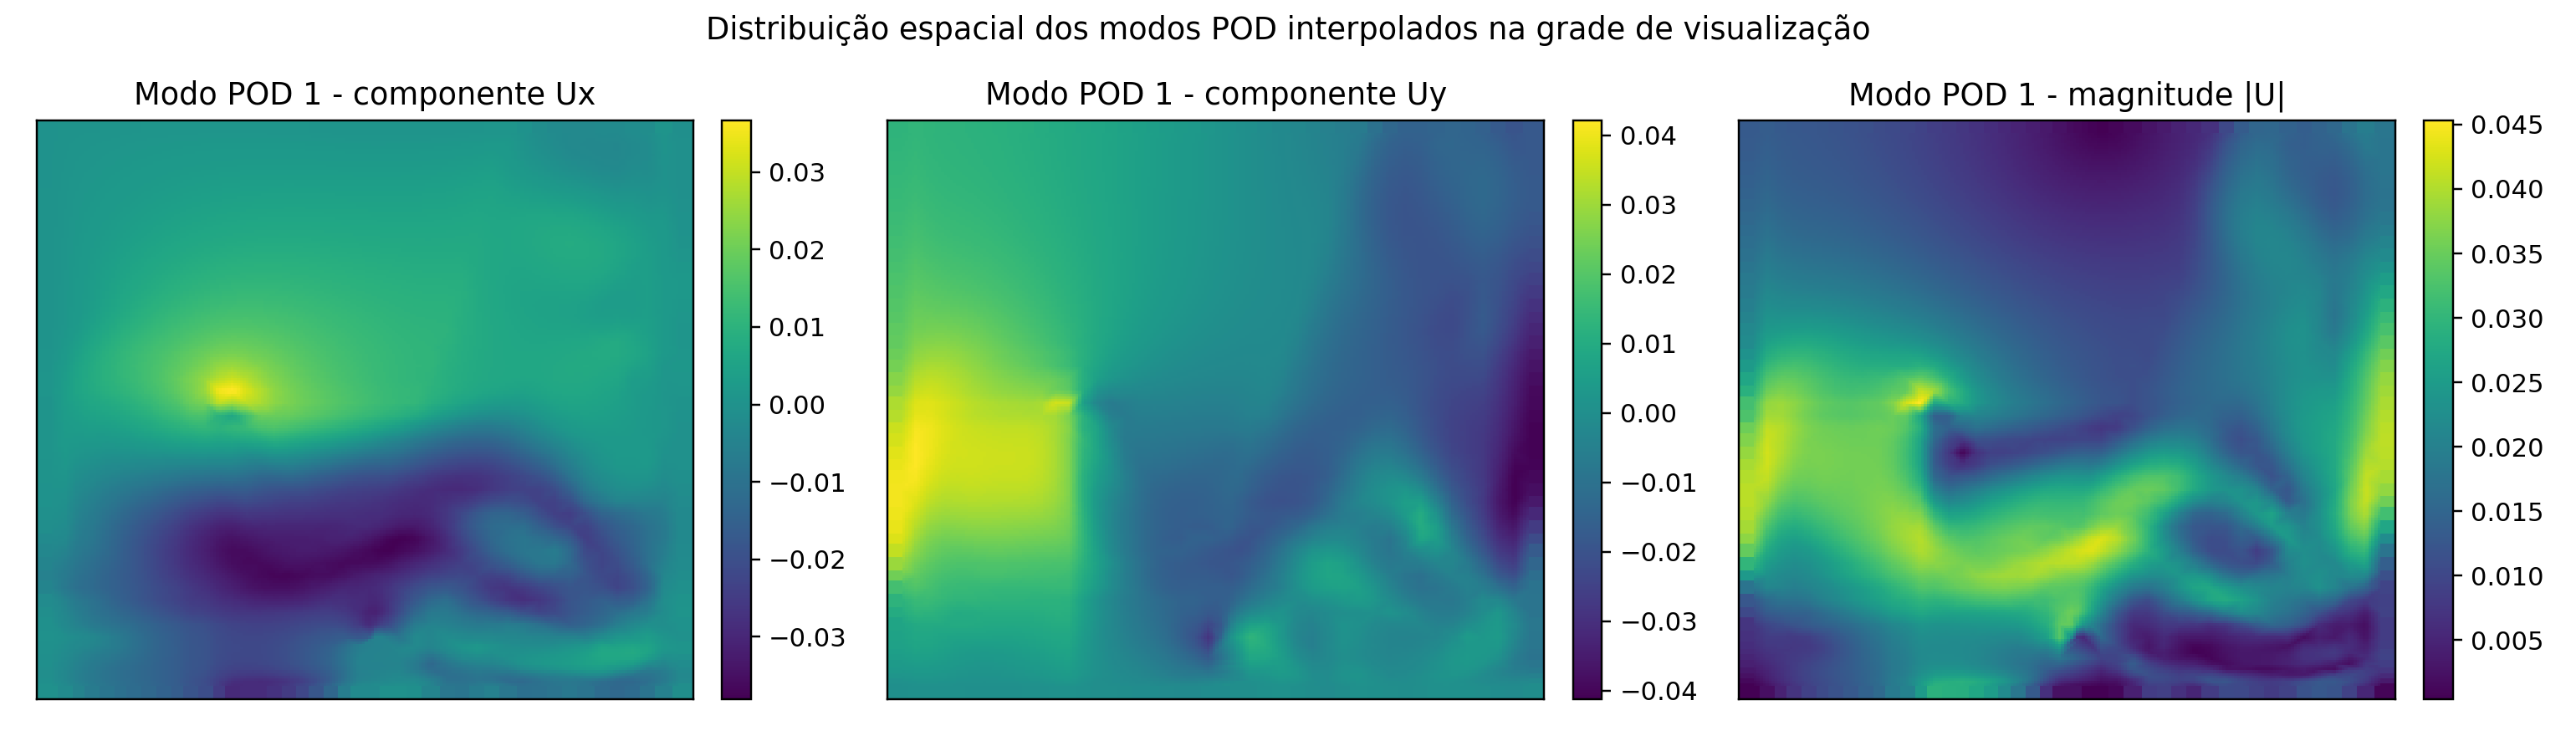
\includegraphics[width=.92\textwidth]{pod_modo1.png}\caption{Primeiro modo POD: $U_x$, $U_y$ e $|U|$.}\end{figure}
\begin{figure}[H]\centering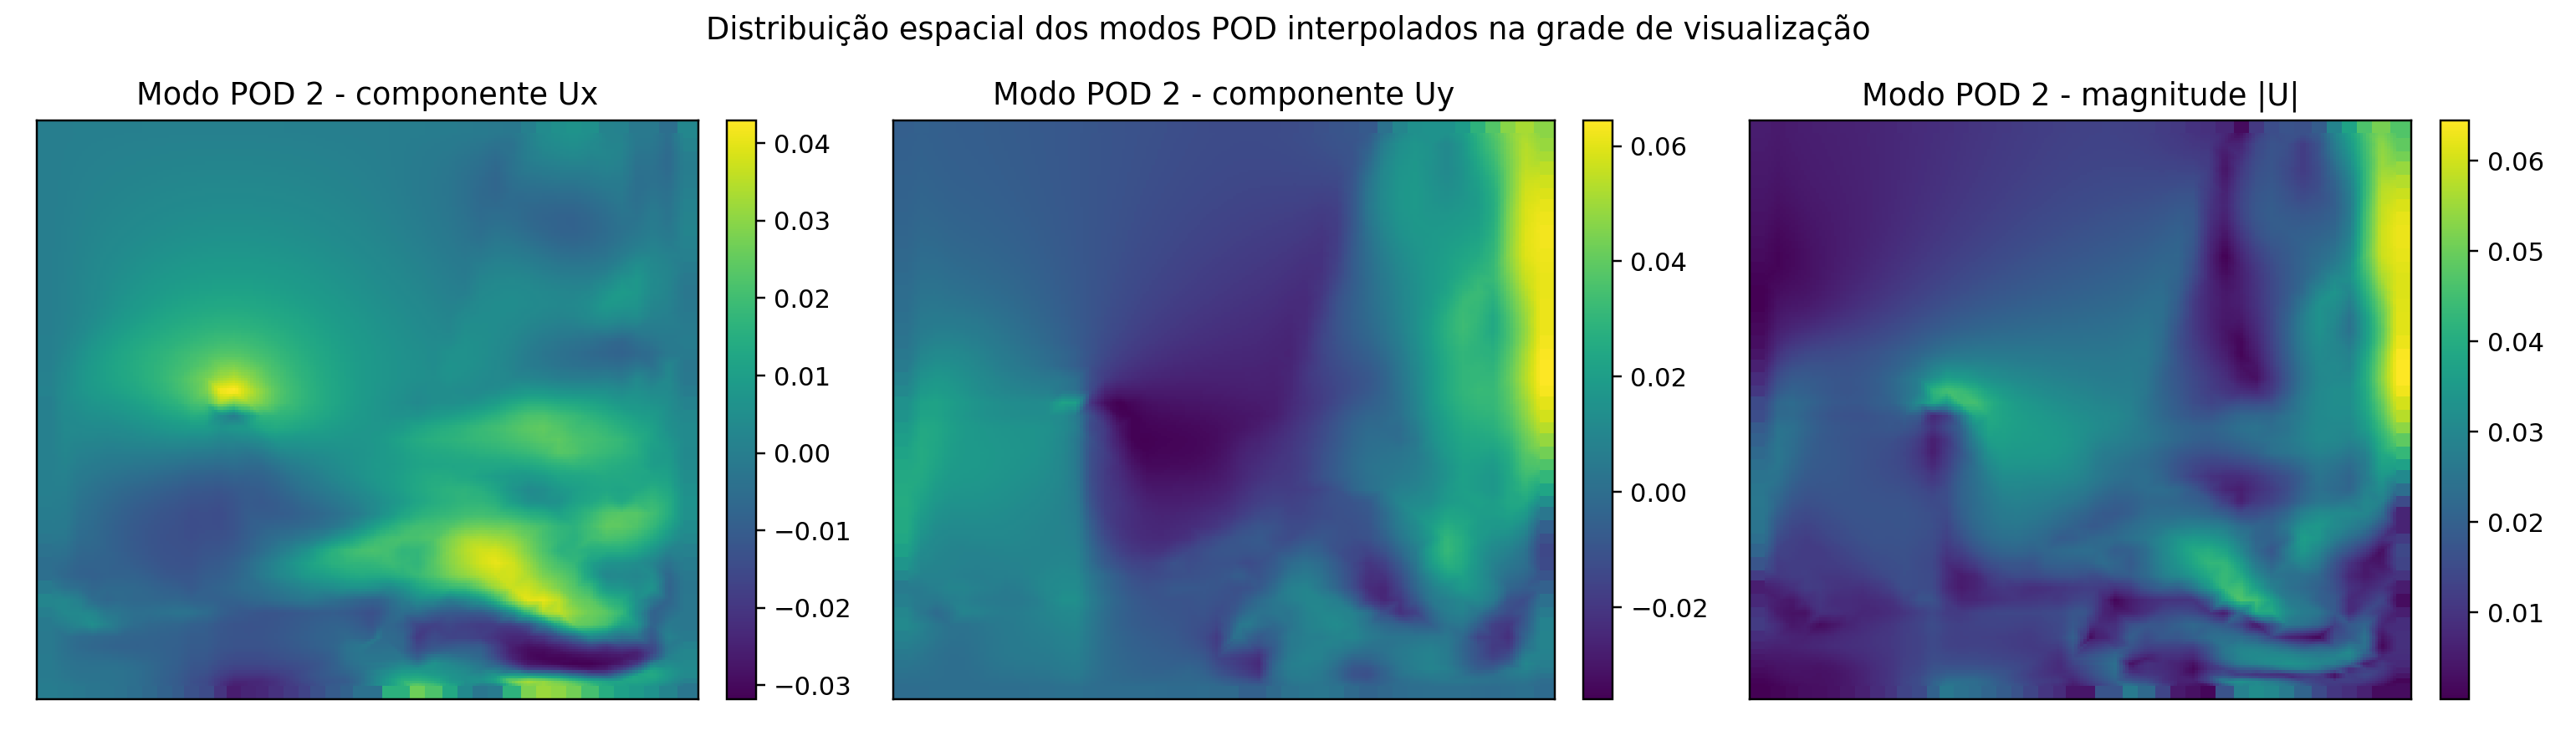
\includegraphics[width=.92\textwidth]{pod_modo2.png}\caption{Segundo modo POD.}\end{figure}
\begin{figure}[H]\centering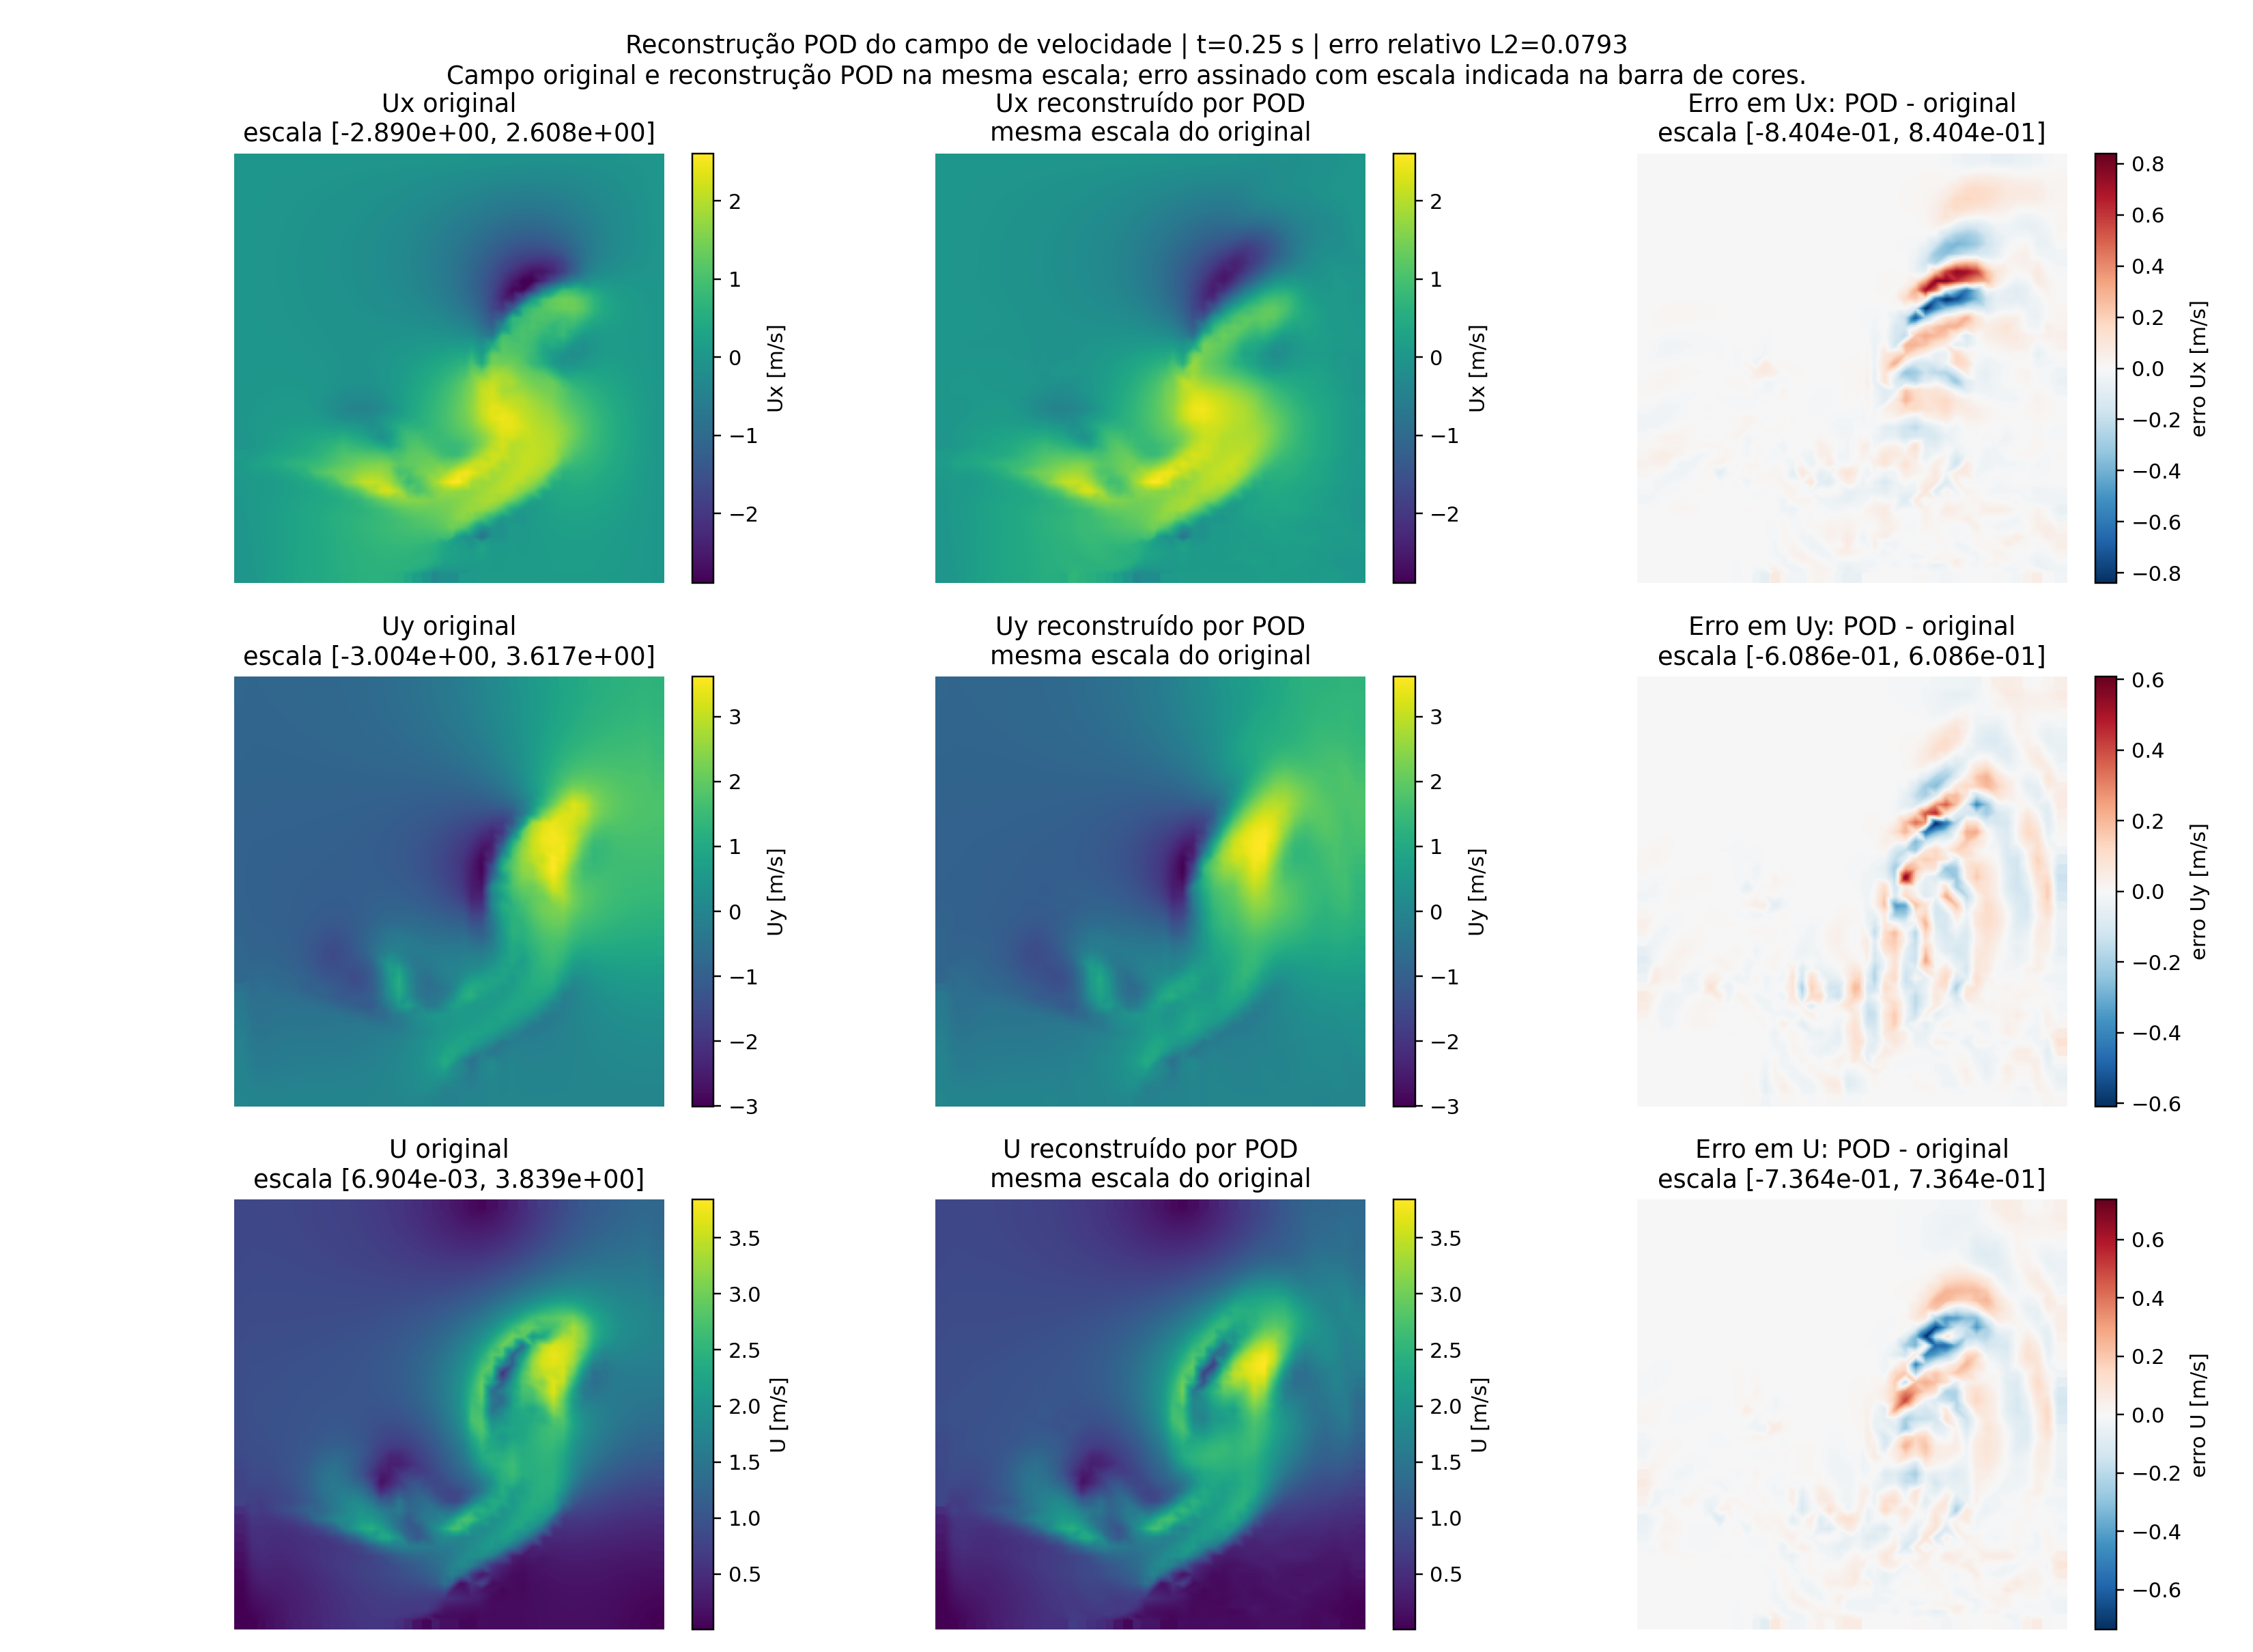
\includegraphics[width=.9\textwidth]{pod_t025.png}\caption{Reconstrução POD isolada em $t=\SI{0.25}{s}$.}\end{figure}
\begin{figure}[H]\centering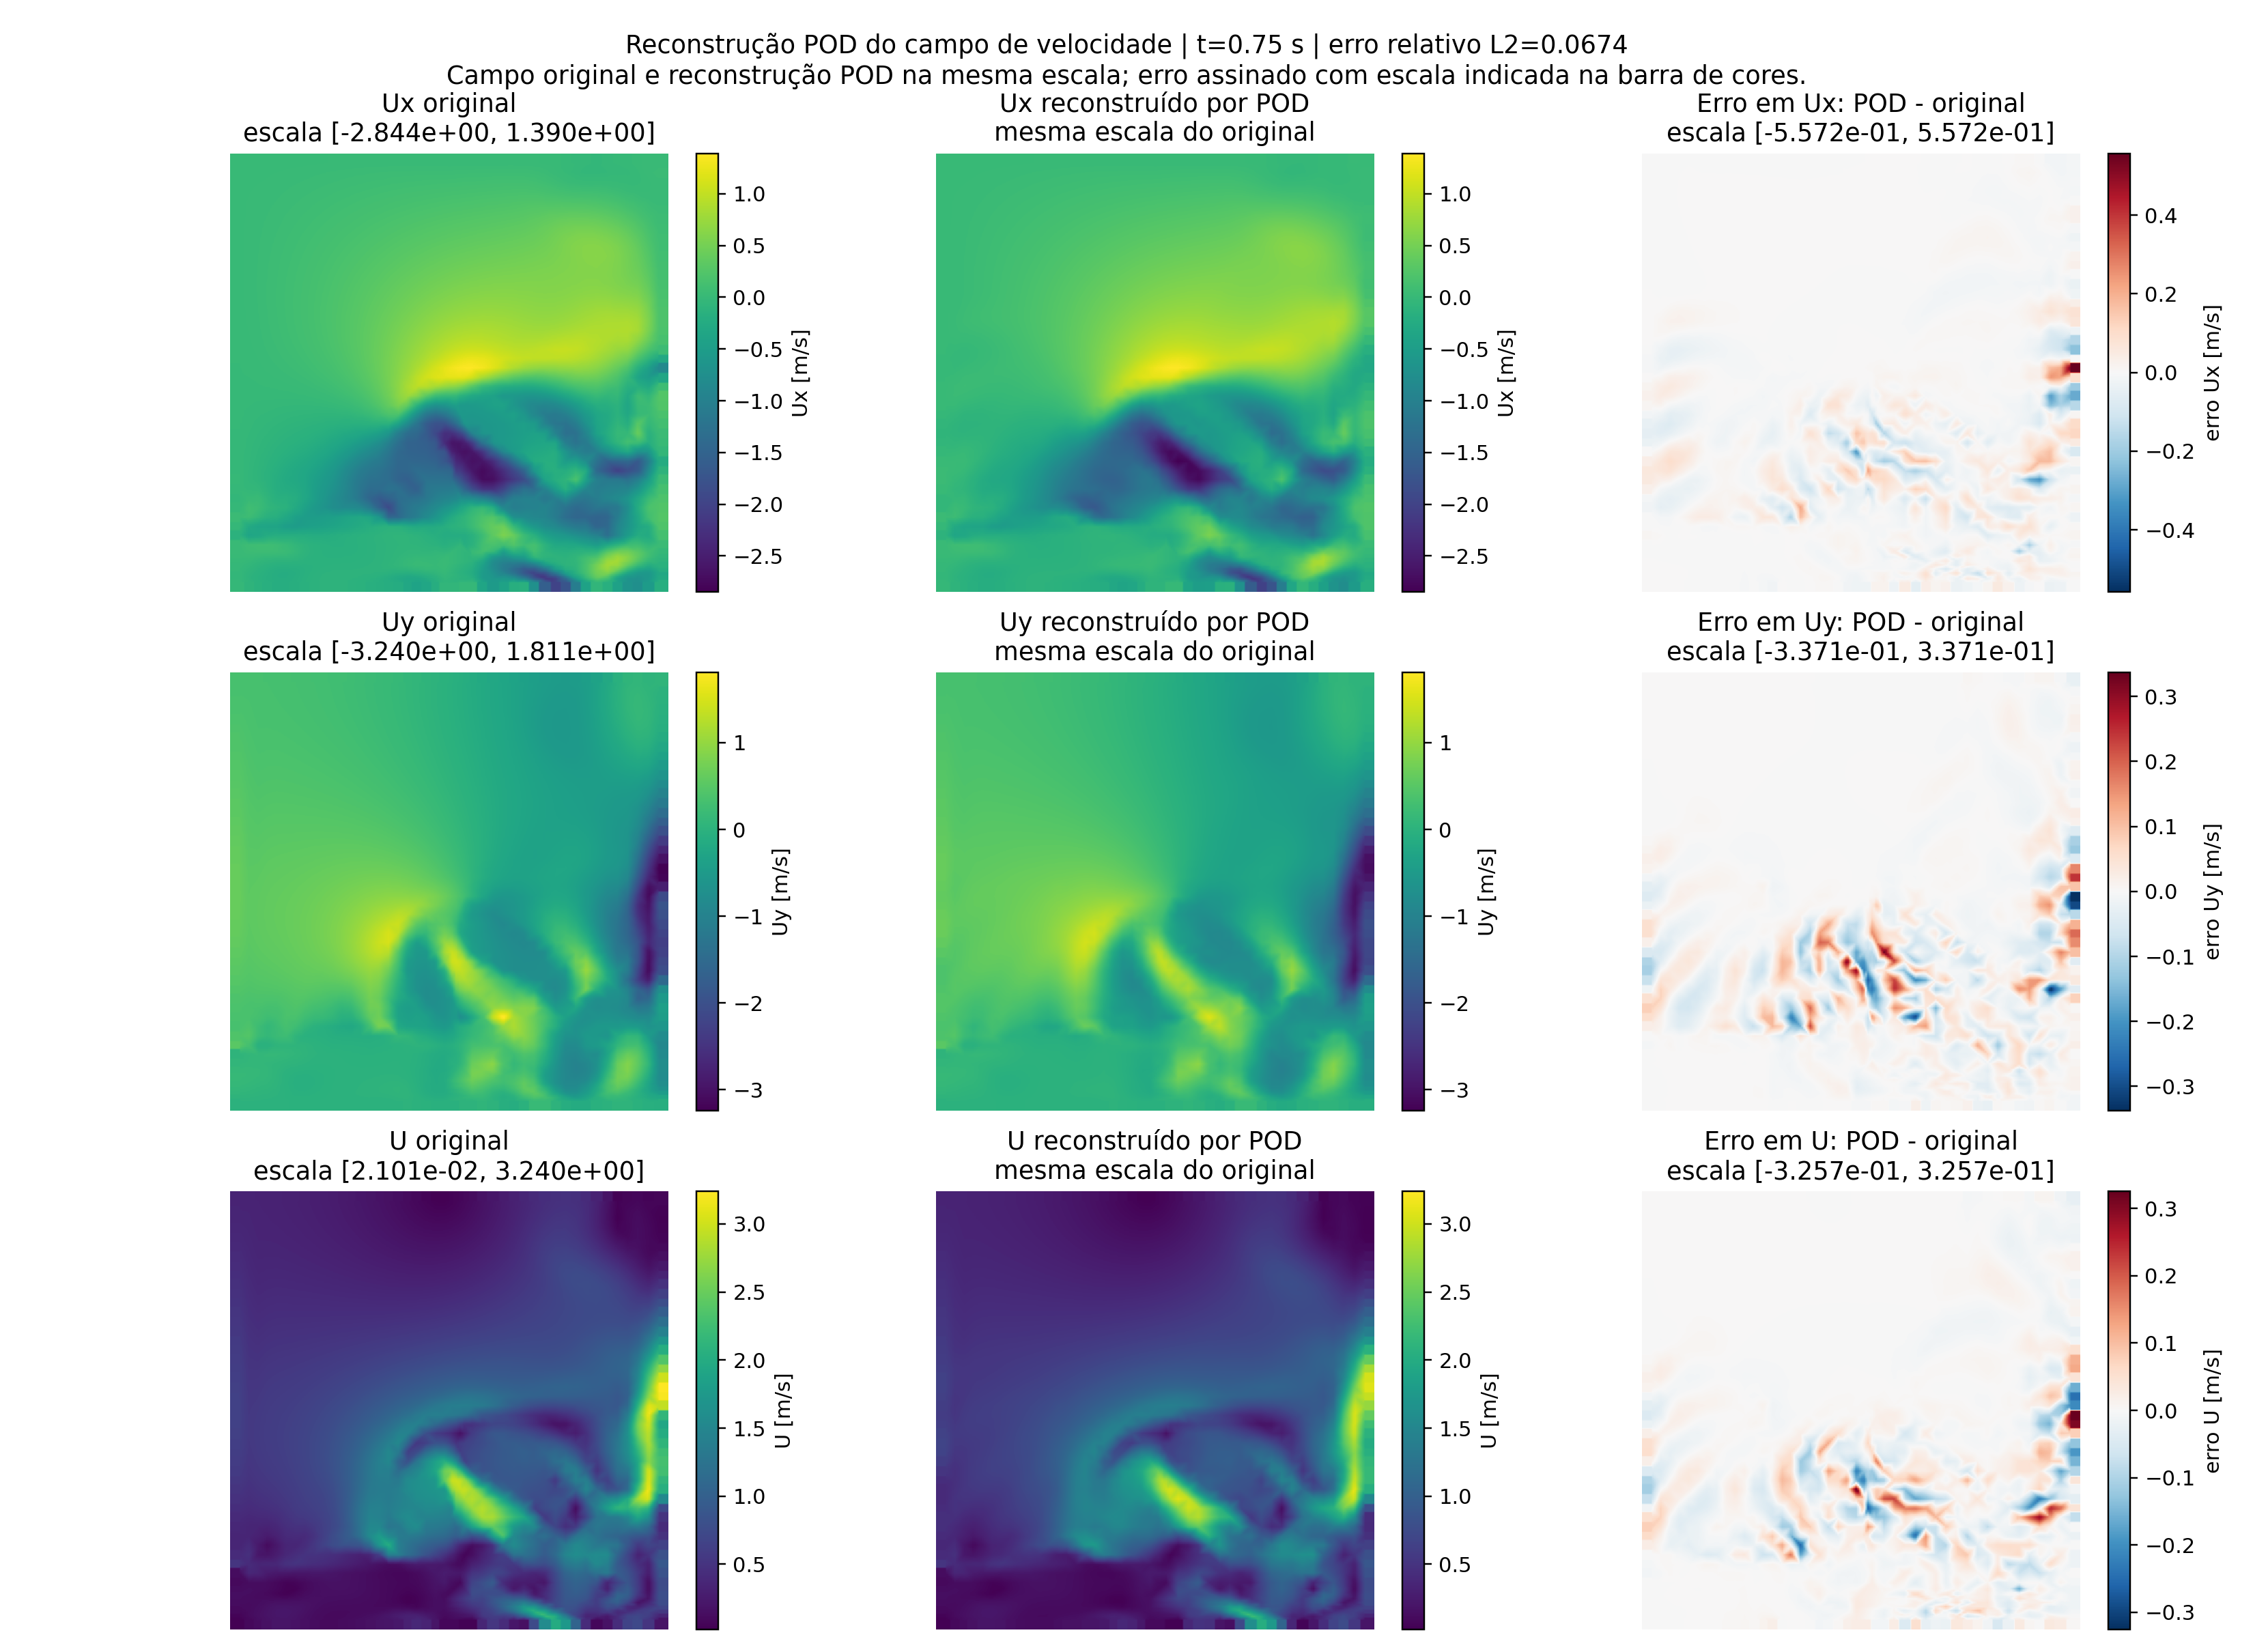
\includegraphics[width=.9\textwidth]{pod_t075.png}\caption{Reconstrução POD isolada em $t=\SI{0.75}{s}$.}\end{figure}

A POD é interpretável e ótima entre bases lineares, mas oito modos---usados no SINDy inicial---retêm 84,62\% da energia e ainda impõem erro de projeção de 39,22\%. Além disso, esta POD descreve apenas velocidade e não a interface, pressão ou turbulência.

\section{SAE multivariável}
O artefato Keras salvo usa entrada $32\times32\times5=5120$ e canais $U_x,U_y,\alpha_{water},p_{rgh},k$. O encoder é 128--64--32--4, com Batch Normalization, e o decoder é simétrico. Foram usados Adam com taxa $5\times10^{-5}$ e perda Huber. O conjunto possui 1001 snapshots obtidos com stride 10 sobre a saída CFD; há 801 amostras de treino e 200 de validação.

\begin{table}[H]\centering
\caption{Parâmetros SAE confirmados nos artefatos.}\label{tab:saeparam}
\begin{tabularx}{\textwidth}{>{\bfseries}l X}
\toprule Parâmetro & Valor\\\midrule
Entrada/canais & 5120; $U_x,U_y,\alpha_{water},p_{rgh},k$\\
Encoder/latente & 128--64--32; dimensão 4 linear\\
Decoder & 32--64--128--5120\\
Otimização & Adam, $5\times10^{-5}$; Huber; 150 épocas registradas; lote declarado 32\\
Normalização & por atributo; pisos de desvio por canal armazenados; corte z-score declarado $\pm4$\\
Amostras & 1001; treino 801, validação 200\\
\bottomrule\end{tabularx}\end{table}

\begin{table}[H]\centering
\caption{Métricas SAE salvas.}\label{tab:saeres}
\begin{tabular}{lrr}\toprule Métrica & Treino & Validação\\\midrule
MSE médio &0,04318&0,04925\\Erro $L_2$ relativo médio&0,23742&0,24090\\$R^2$ global&0,94883&0,94183\\\bottomrule\end{tabular}\end{table}
A melhor época registrada é 148 e a menor perda de validação é 0,01951. A proximidade entre treino e validação é positiva, mas a distribuição temporal dos dois subconjuntos nos NPZ não coincide com o split temporal escrito atualmente no notebook; logo, o resultado mede interpolação entre estados distribuídos no tempo mais do que extrapolação temporal.

\begin{figure}[H]\centering
\begin{subfigure}{.49\textwidth}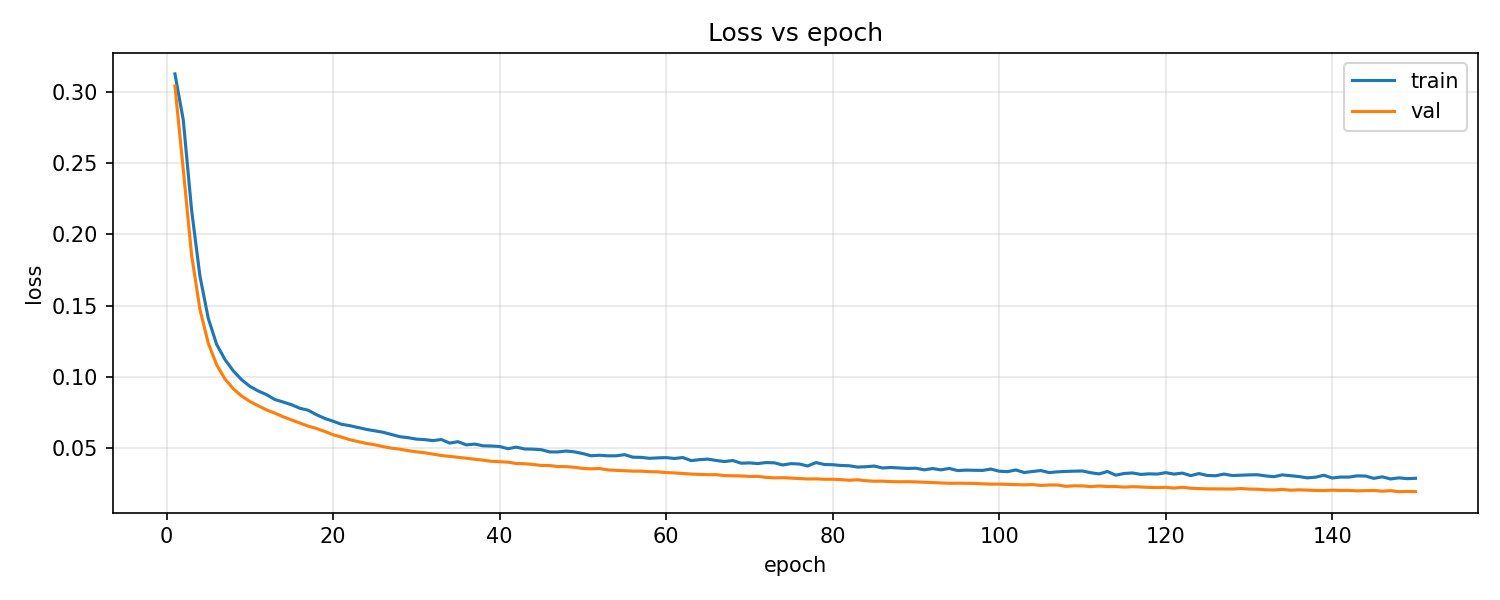
\includegraphics[width=\linewidth]{sae_loss.png}\caption{Perdas.}\end{subfigure}
\begin{subfigure}{.49\textwidth}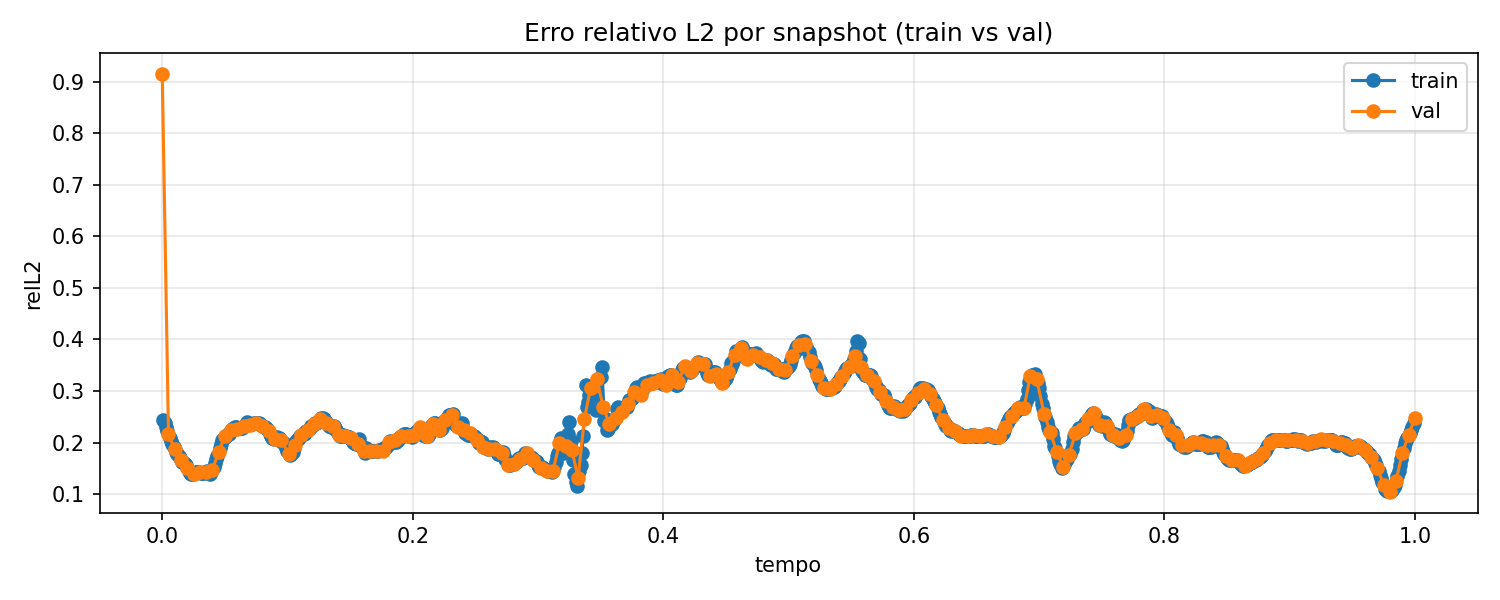
\includegraphics[width=\linewidth]{sae_rel.png}\caption{Erro por snapshot.}\end{subfigure}
\caption{Diagnóstico do SAE.}\end{figure}
\begin{figure}[H]\centering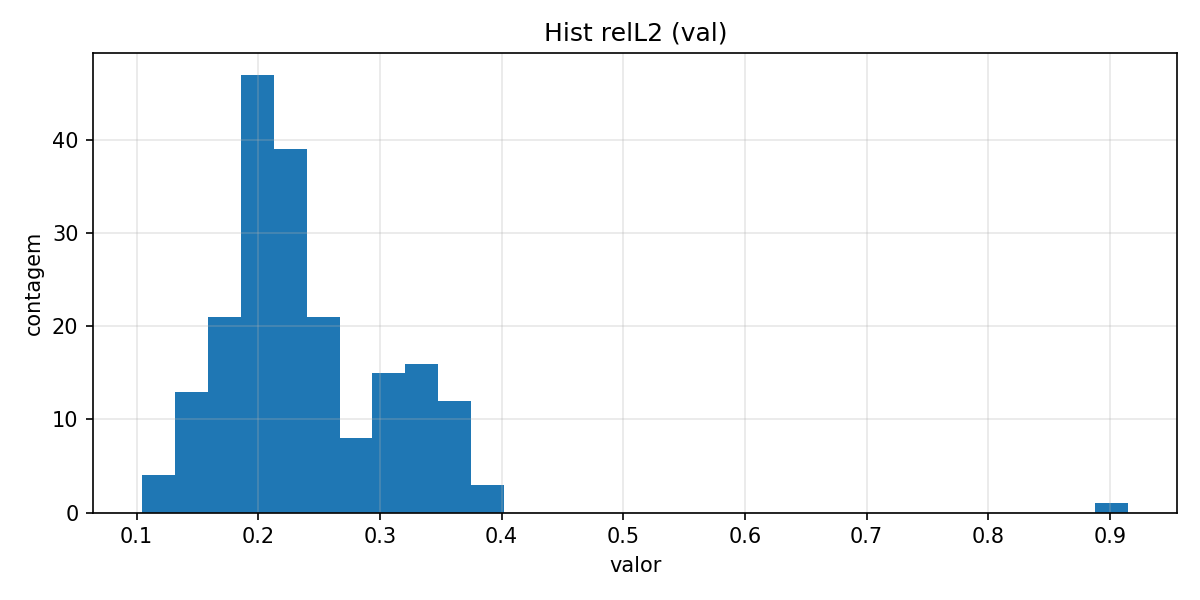
\includegraphics[width=.62\textwidth]{sae_hist.png}\caption{Histograma do erro relativo de validação.}\end{figure}
\begin{figure}[H]\centering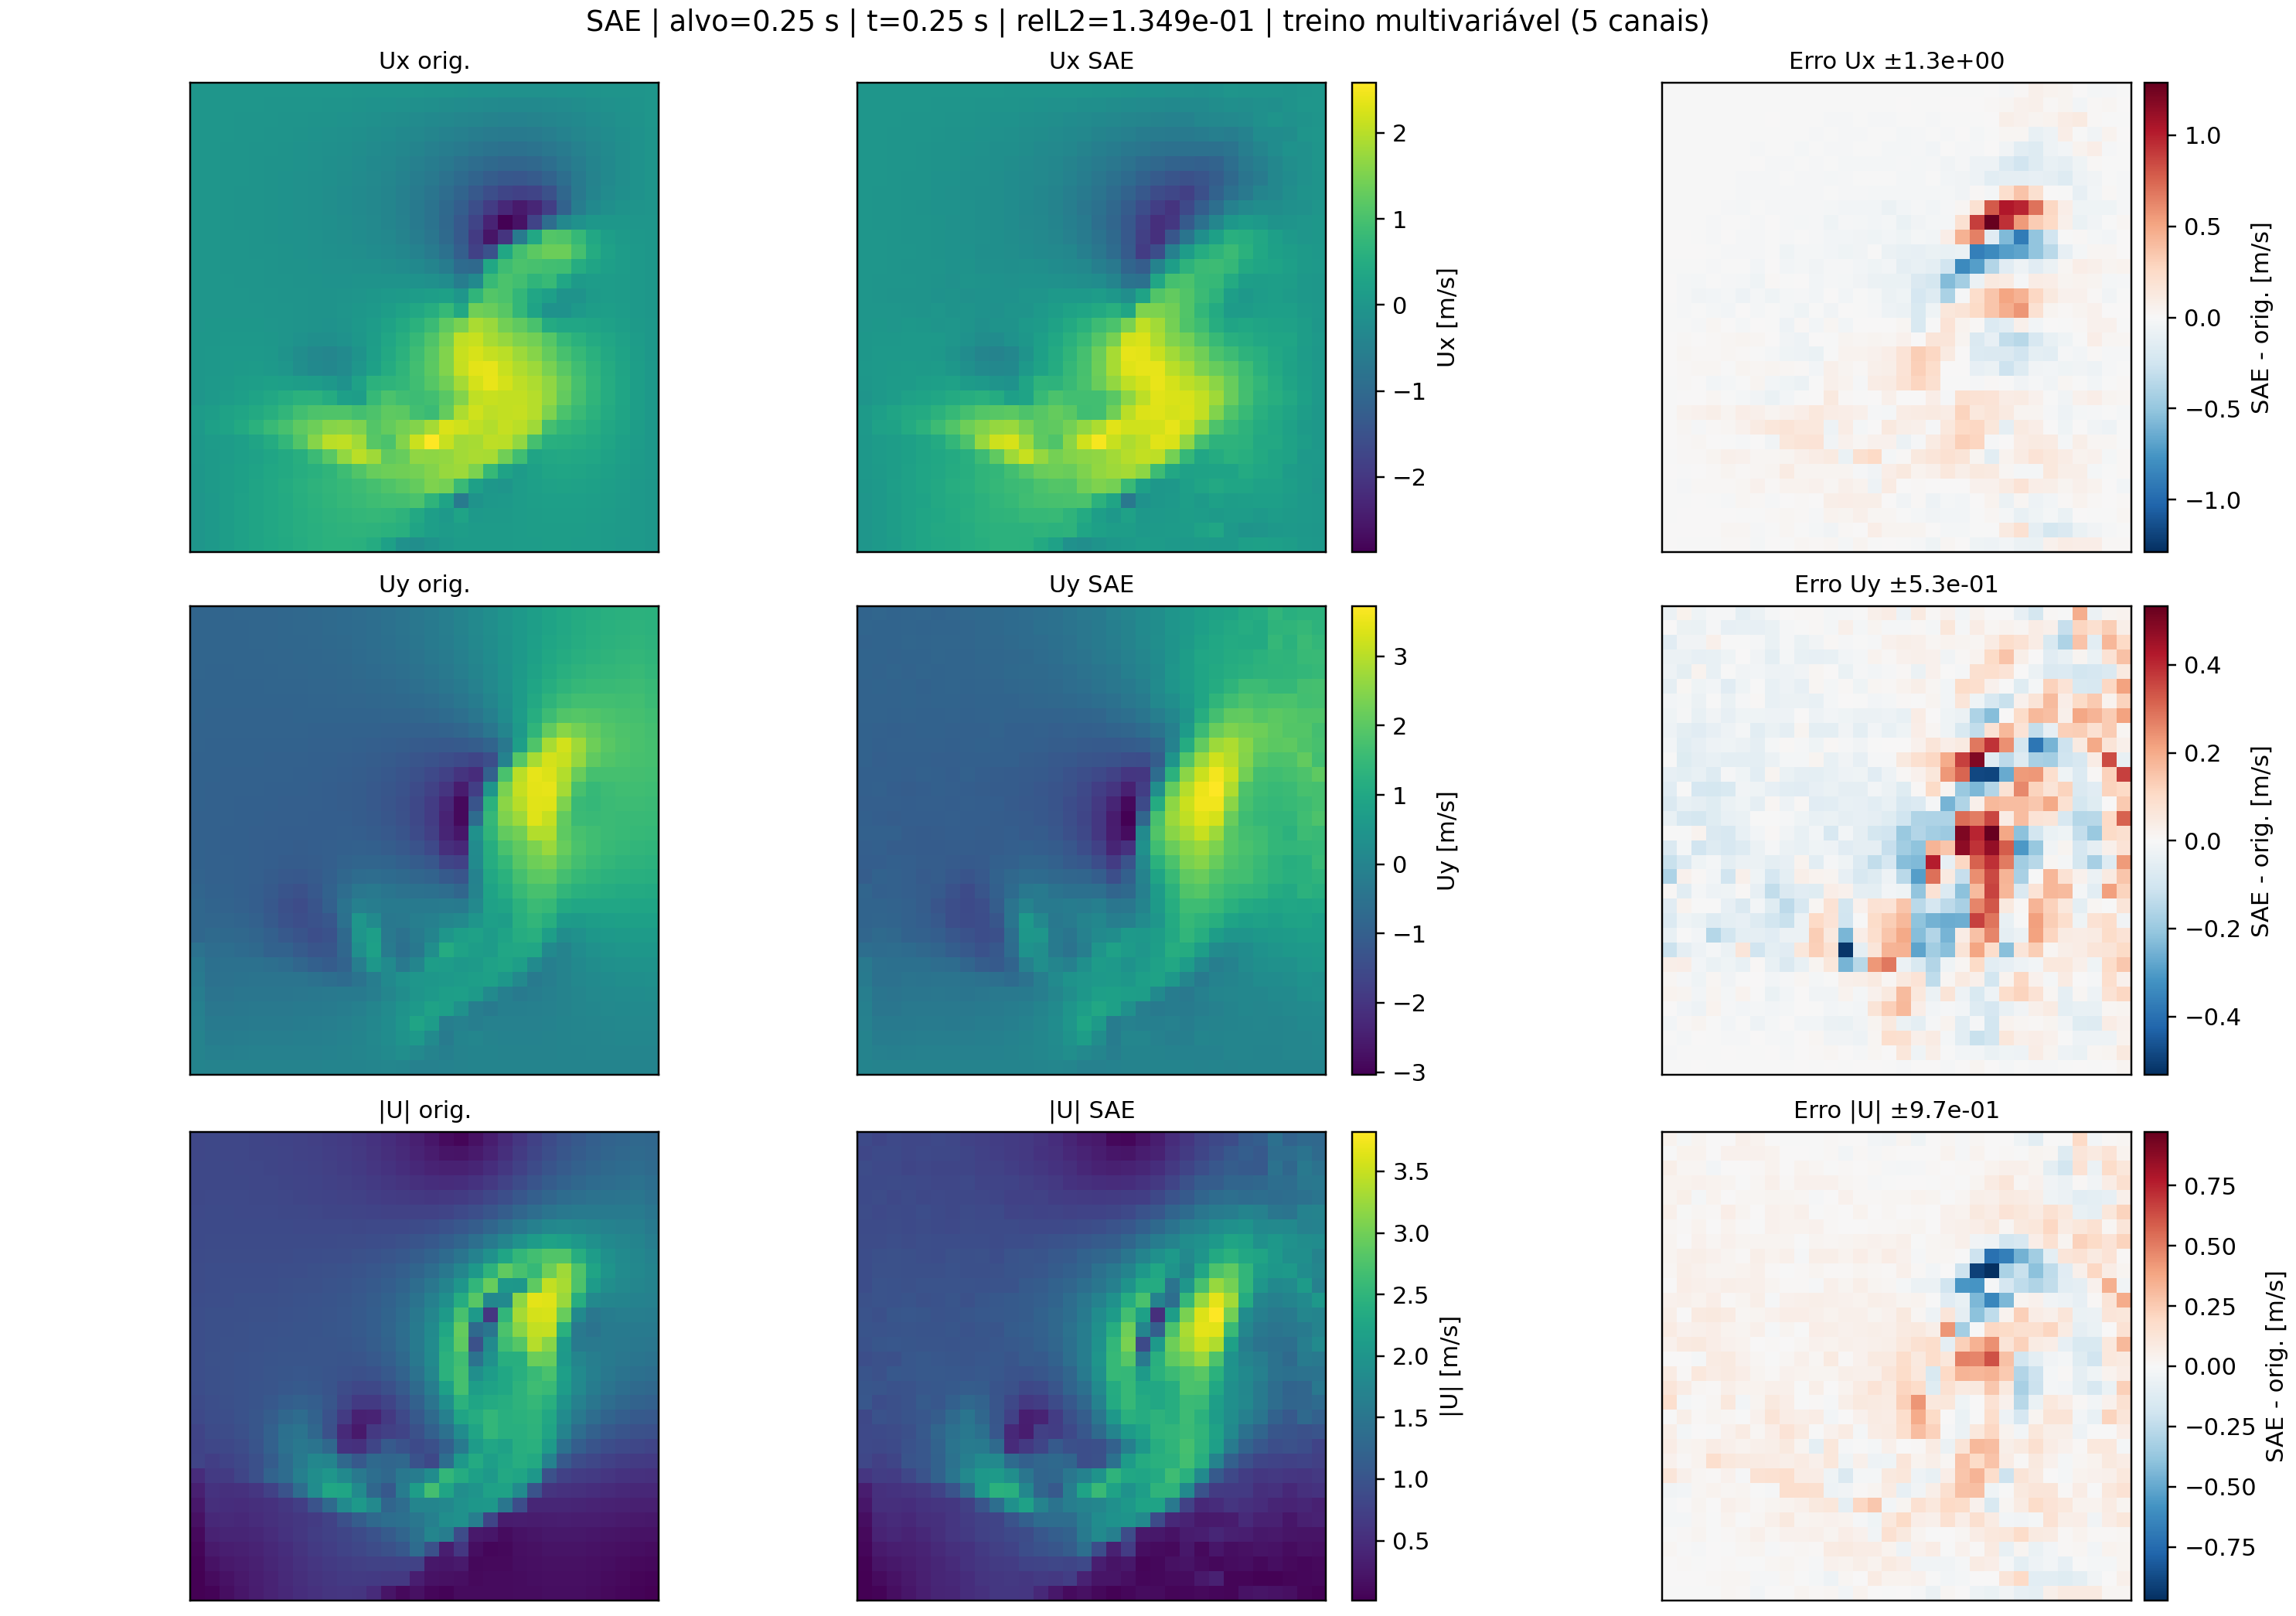
\includegraphics[width=.92\textwidth]{sae_t025.png}\caption{Reconstrução SAE isolada em $t=\SI{0.25}{s}$.}\end{figure}
\begin{figure}[H]\centering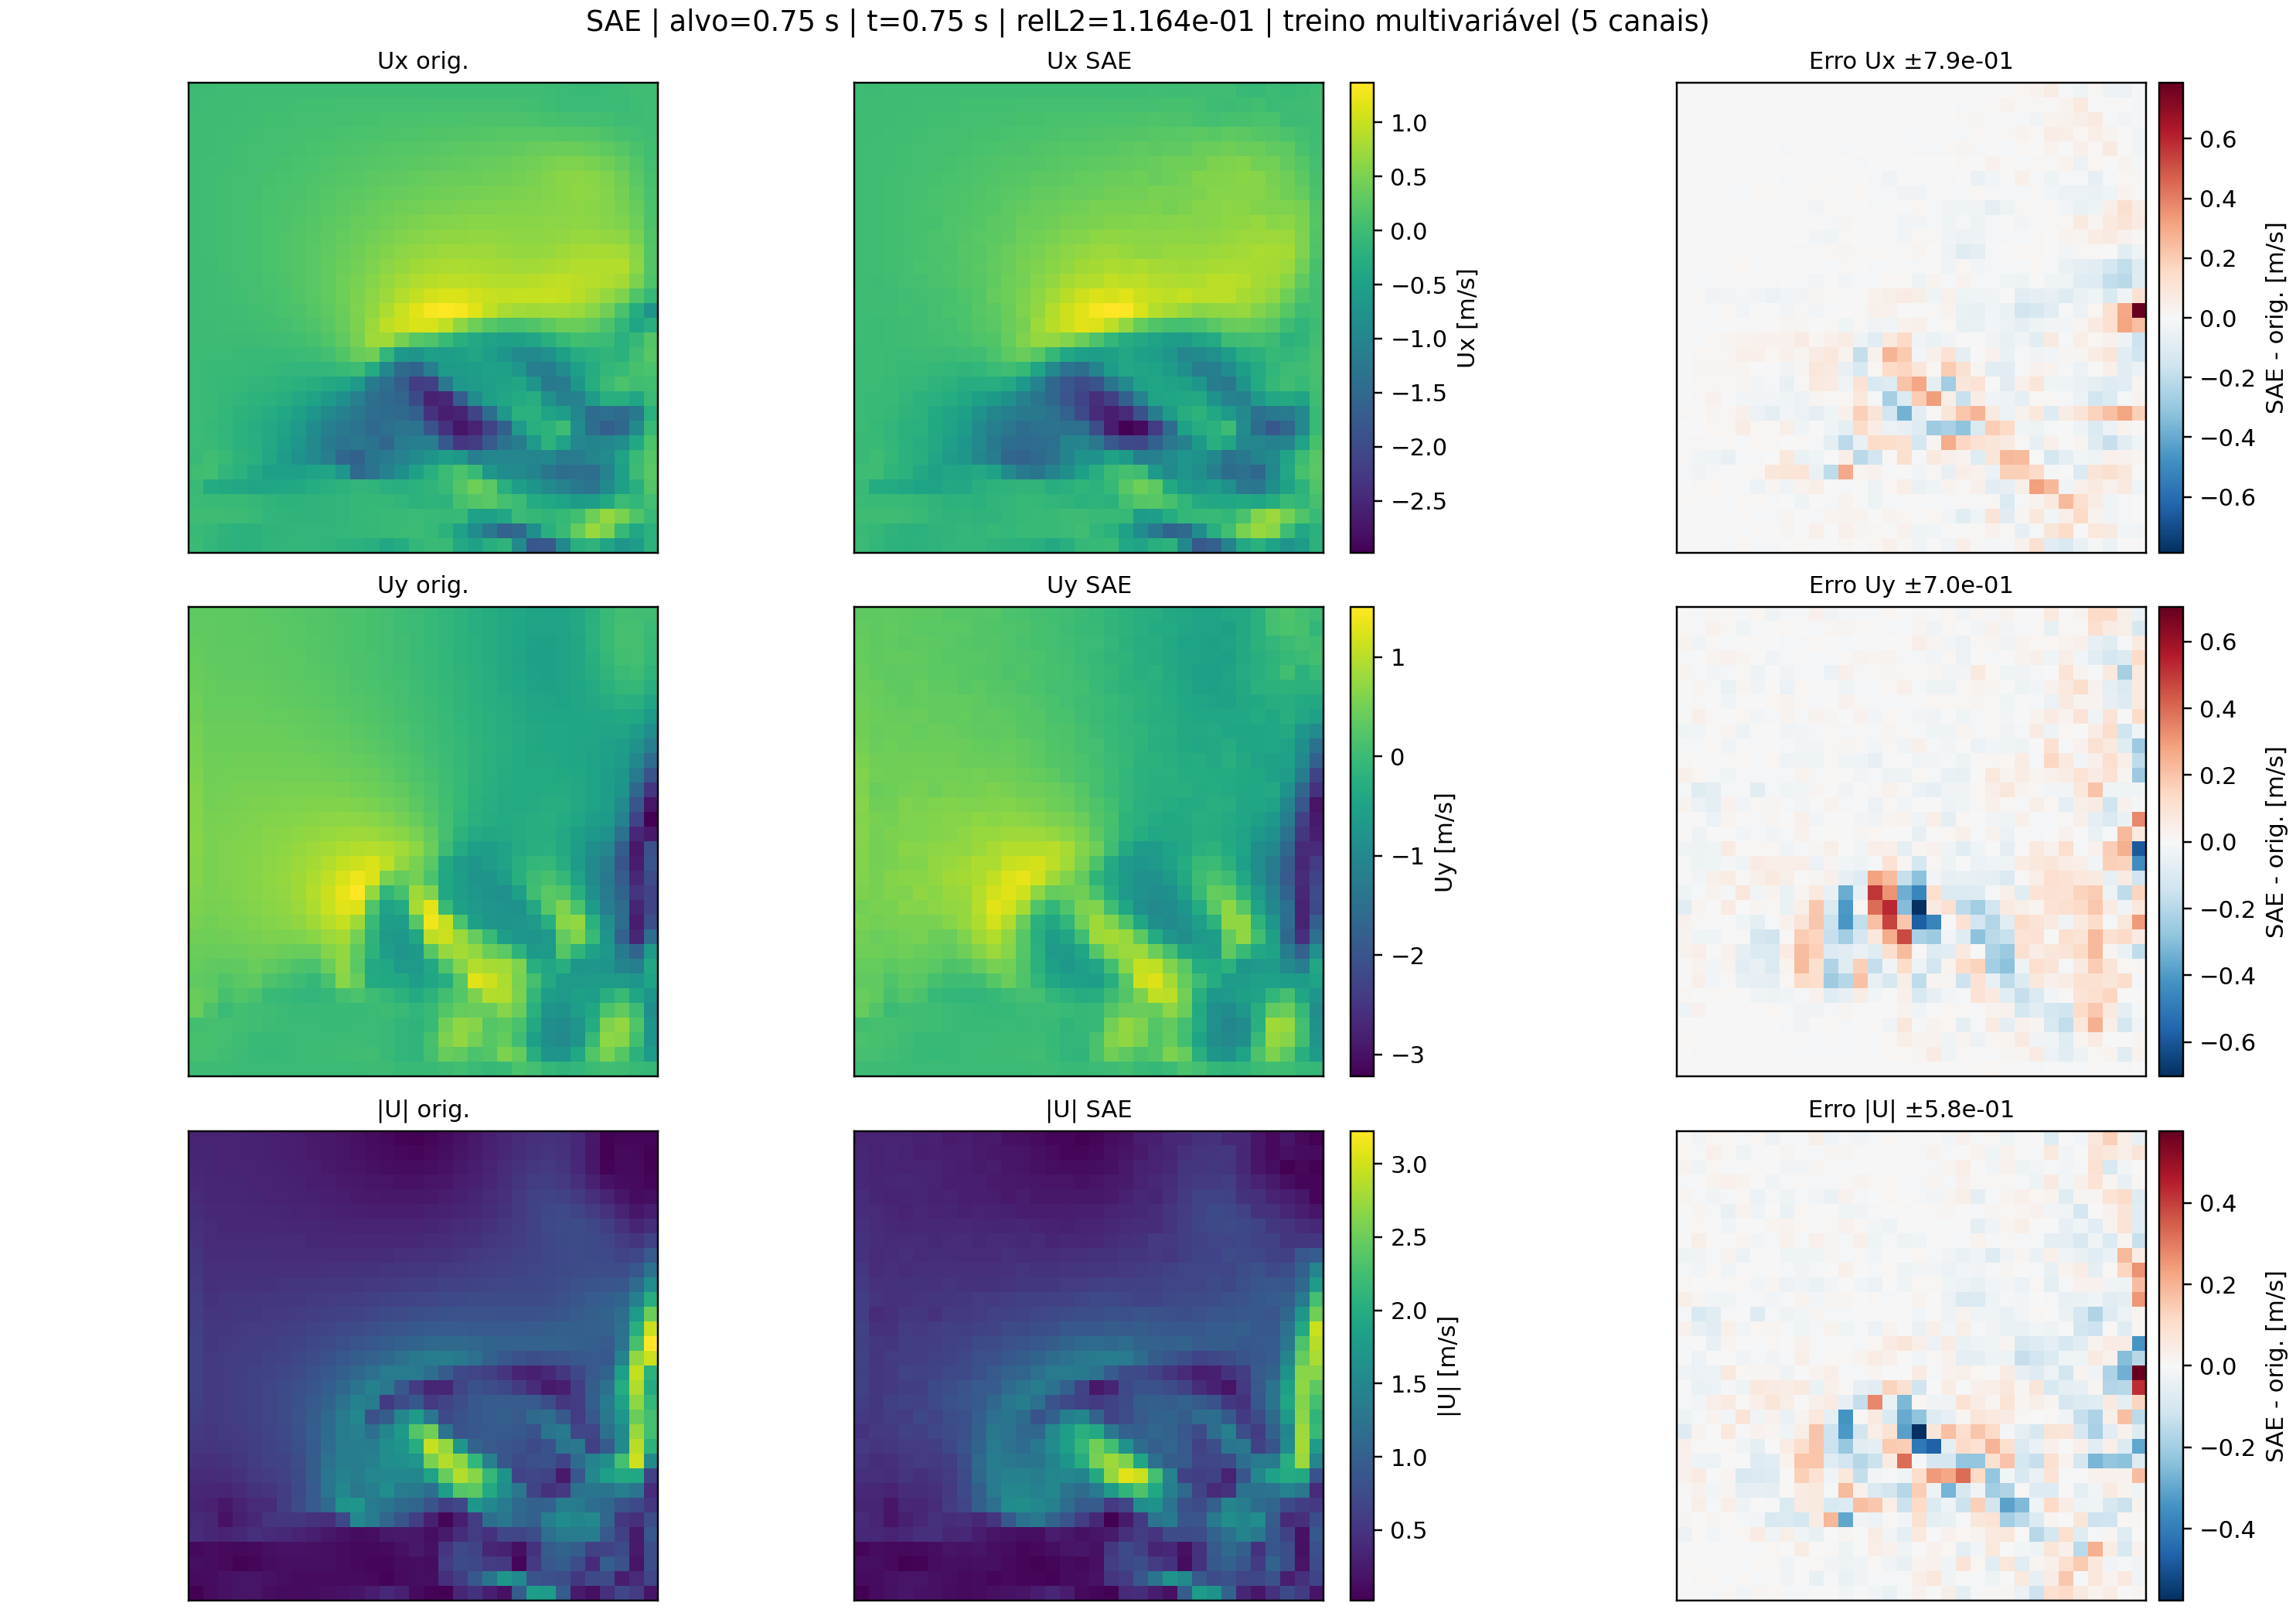
\includegraphics[width=.92\textwidth]{sae_t075.png}\caption{Reconstrução SAE isolada em $t=\SI{0.75}{s}$.}\end{figure}

O SAE captura uma variedade espacial não linear e comprime 5120 valores em quatro latentes. Entretanto, reconstrução não define uma lei temporal: isoladamente, o SAE representa dados, não prevê dinâmica.

\section{SINDy e equações descobertas}
SINDy procura $\dot q=\Theta(q,t)\Xi$. Ajuste de derivadas e erro de um passo são testes locais; integração livre é o teste dinâmico, porque o estado previsto realimenta continuamente as equações.

\subsection{POD--SINDy}
O modelo principal usa oito amplitudes POD, polinômios até ordem 2, sem seno, Lasso com $\alpha=10^{-4}$ e biblioteca de 45 termos. Há 292 coeficientes não nulos em 360 possíveis. O erro de derivada é 0,7836. A integração livre falhou e o erro de trajetória reportado, 0,00300, é de um passo guiado pela referência; não é previsão autônoma.

\lstinputlisting[style=sindyeq,caption={Equações completas POD--SINDy.}]{equacoes_pod_sindy.txt}
\begin{figure}[H]\centering
\begin{subfigure}{.49\textwidth}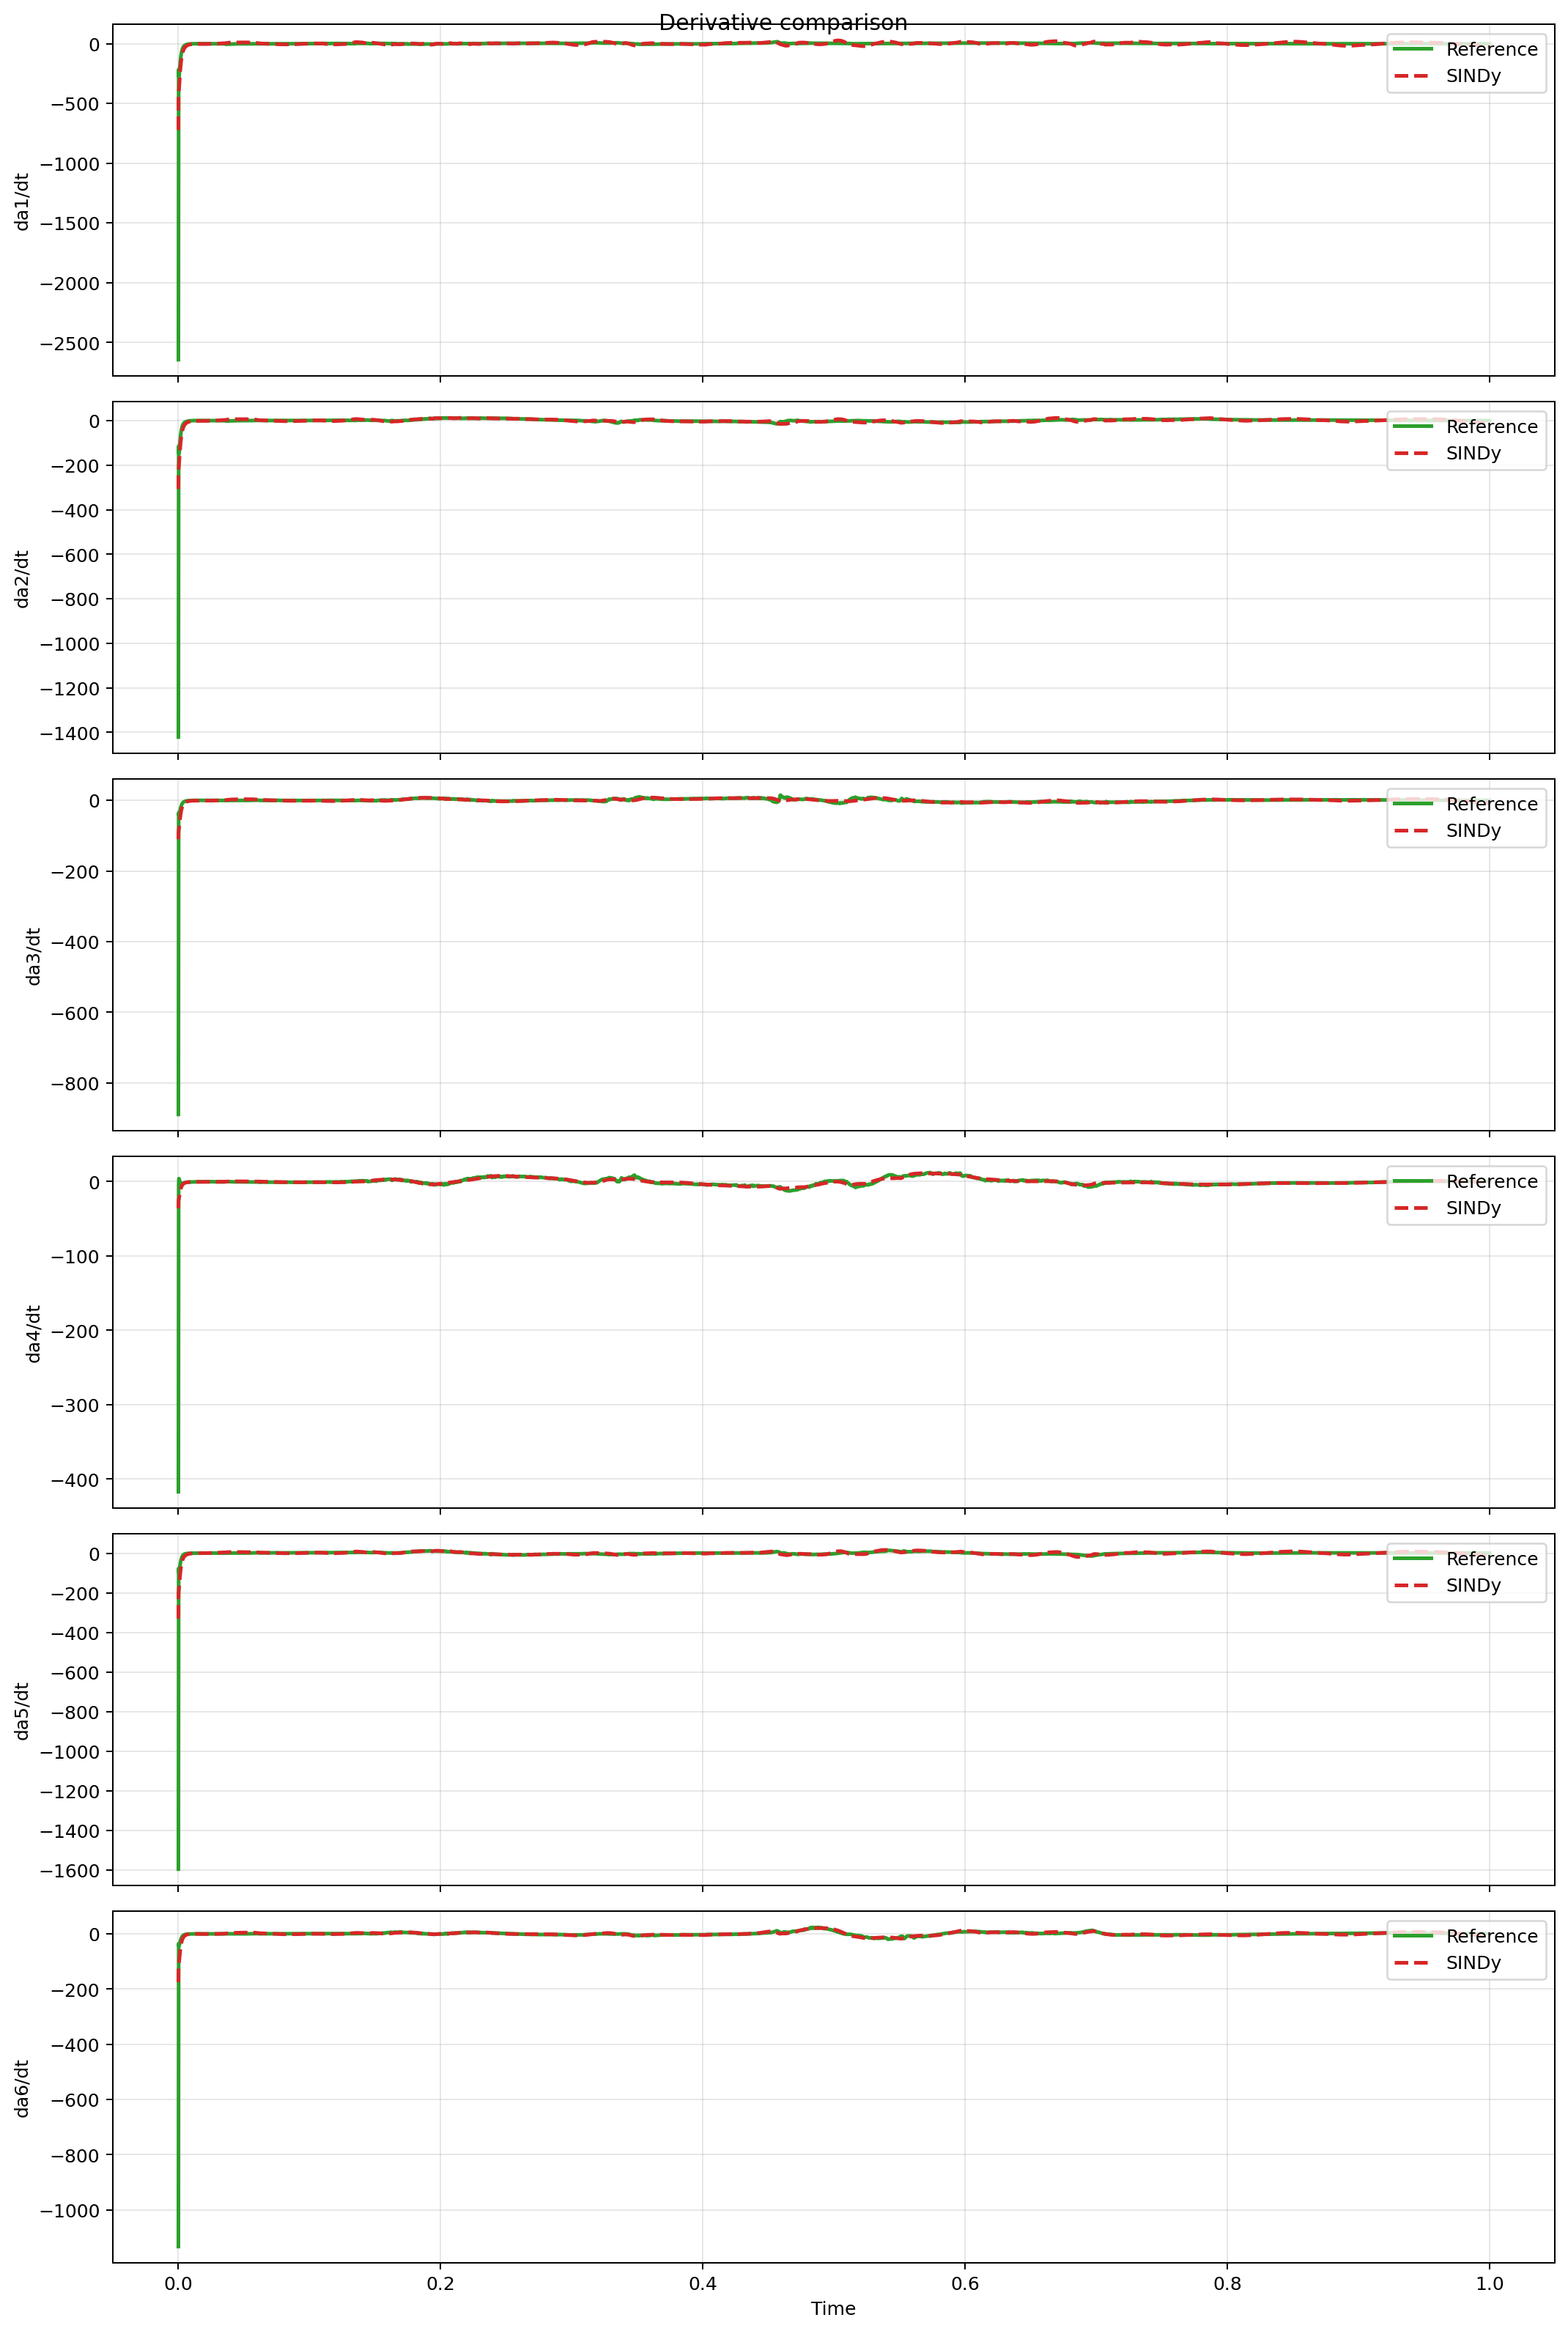
\includegraphics[width=\linewidth]{pods_deriv.png}\caption{Derivadas.}\end{subfigure}
\begin{subfigure}{.49\textwidth}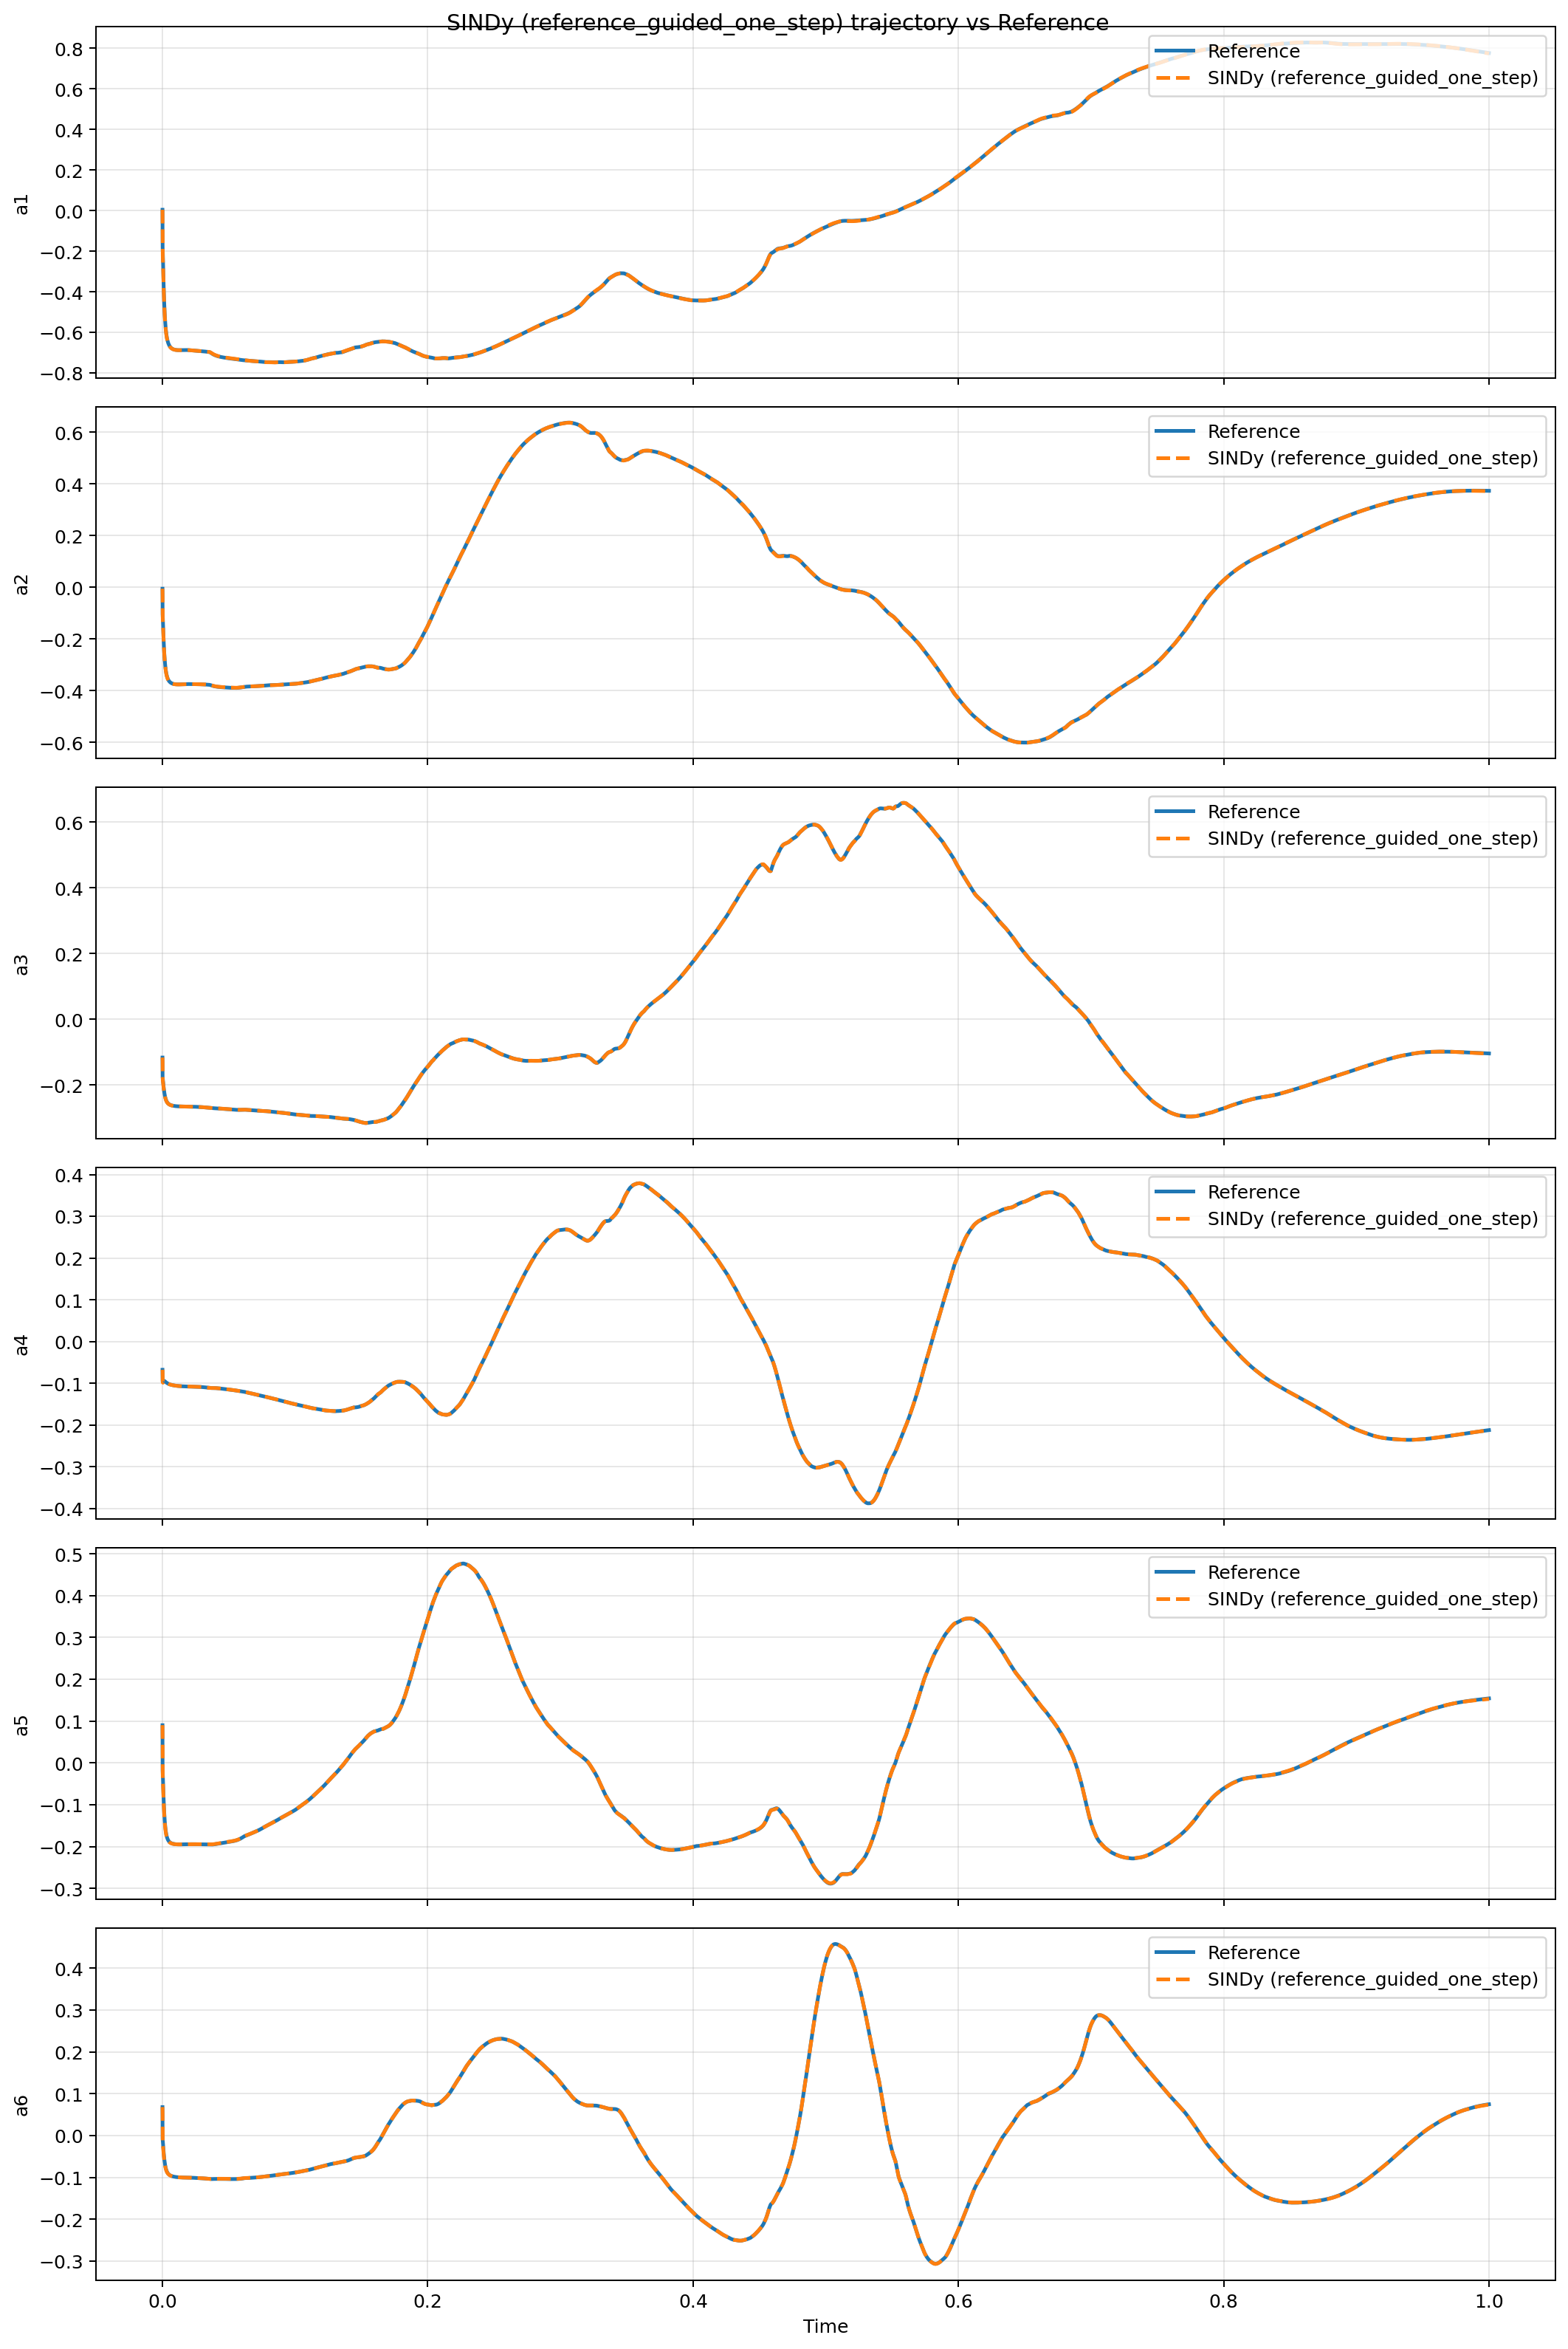
\includegraphics[width=\linewidth]{pods_traj.png}\caption{Trajetória guiada.}\end{subfigure}
\caption{POD--SINDy: ajuste local e falha da integração livre.}\end{figure}
\begin{figure}[H]\centering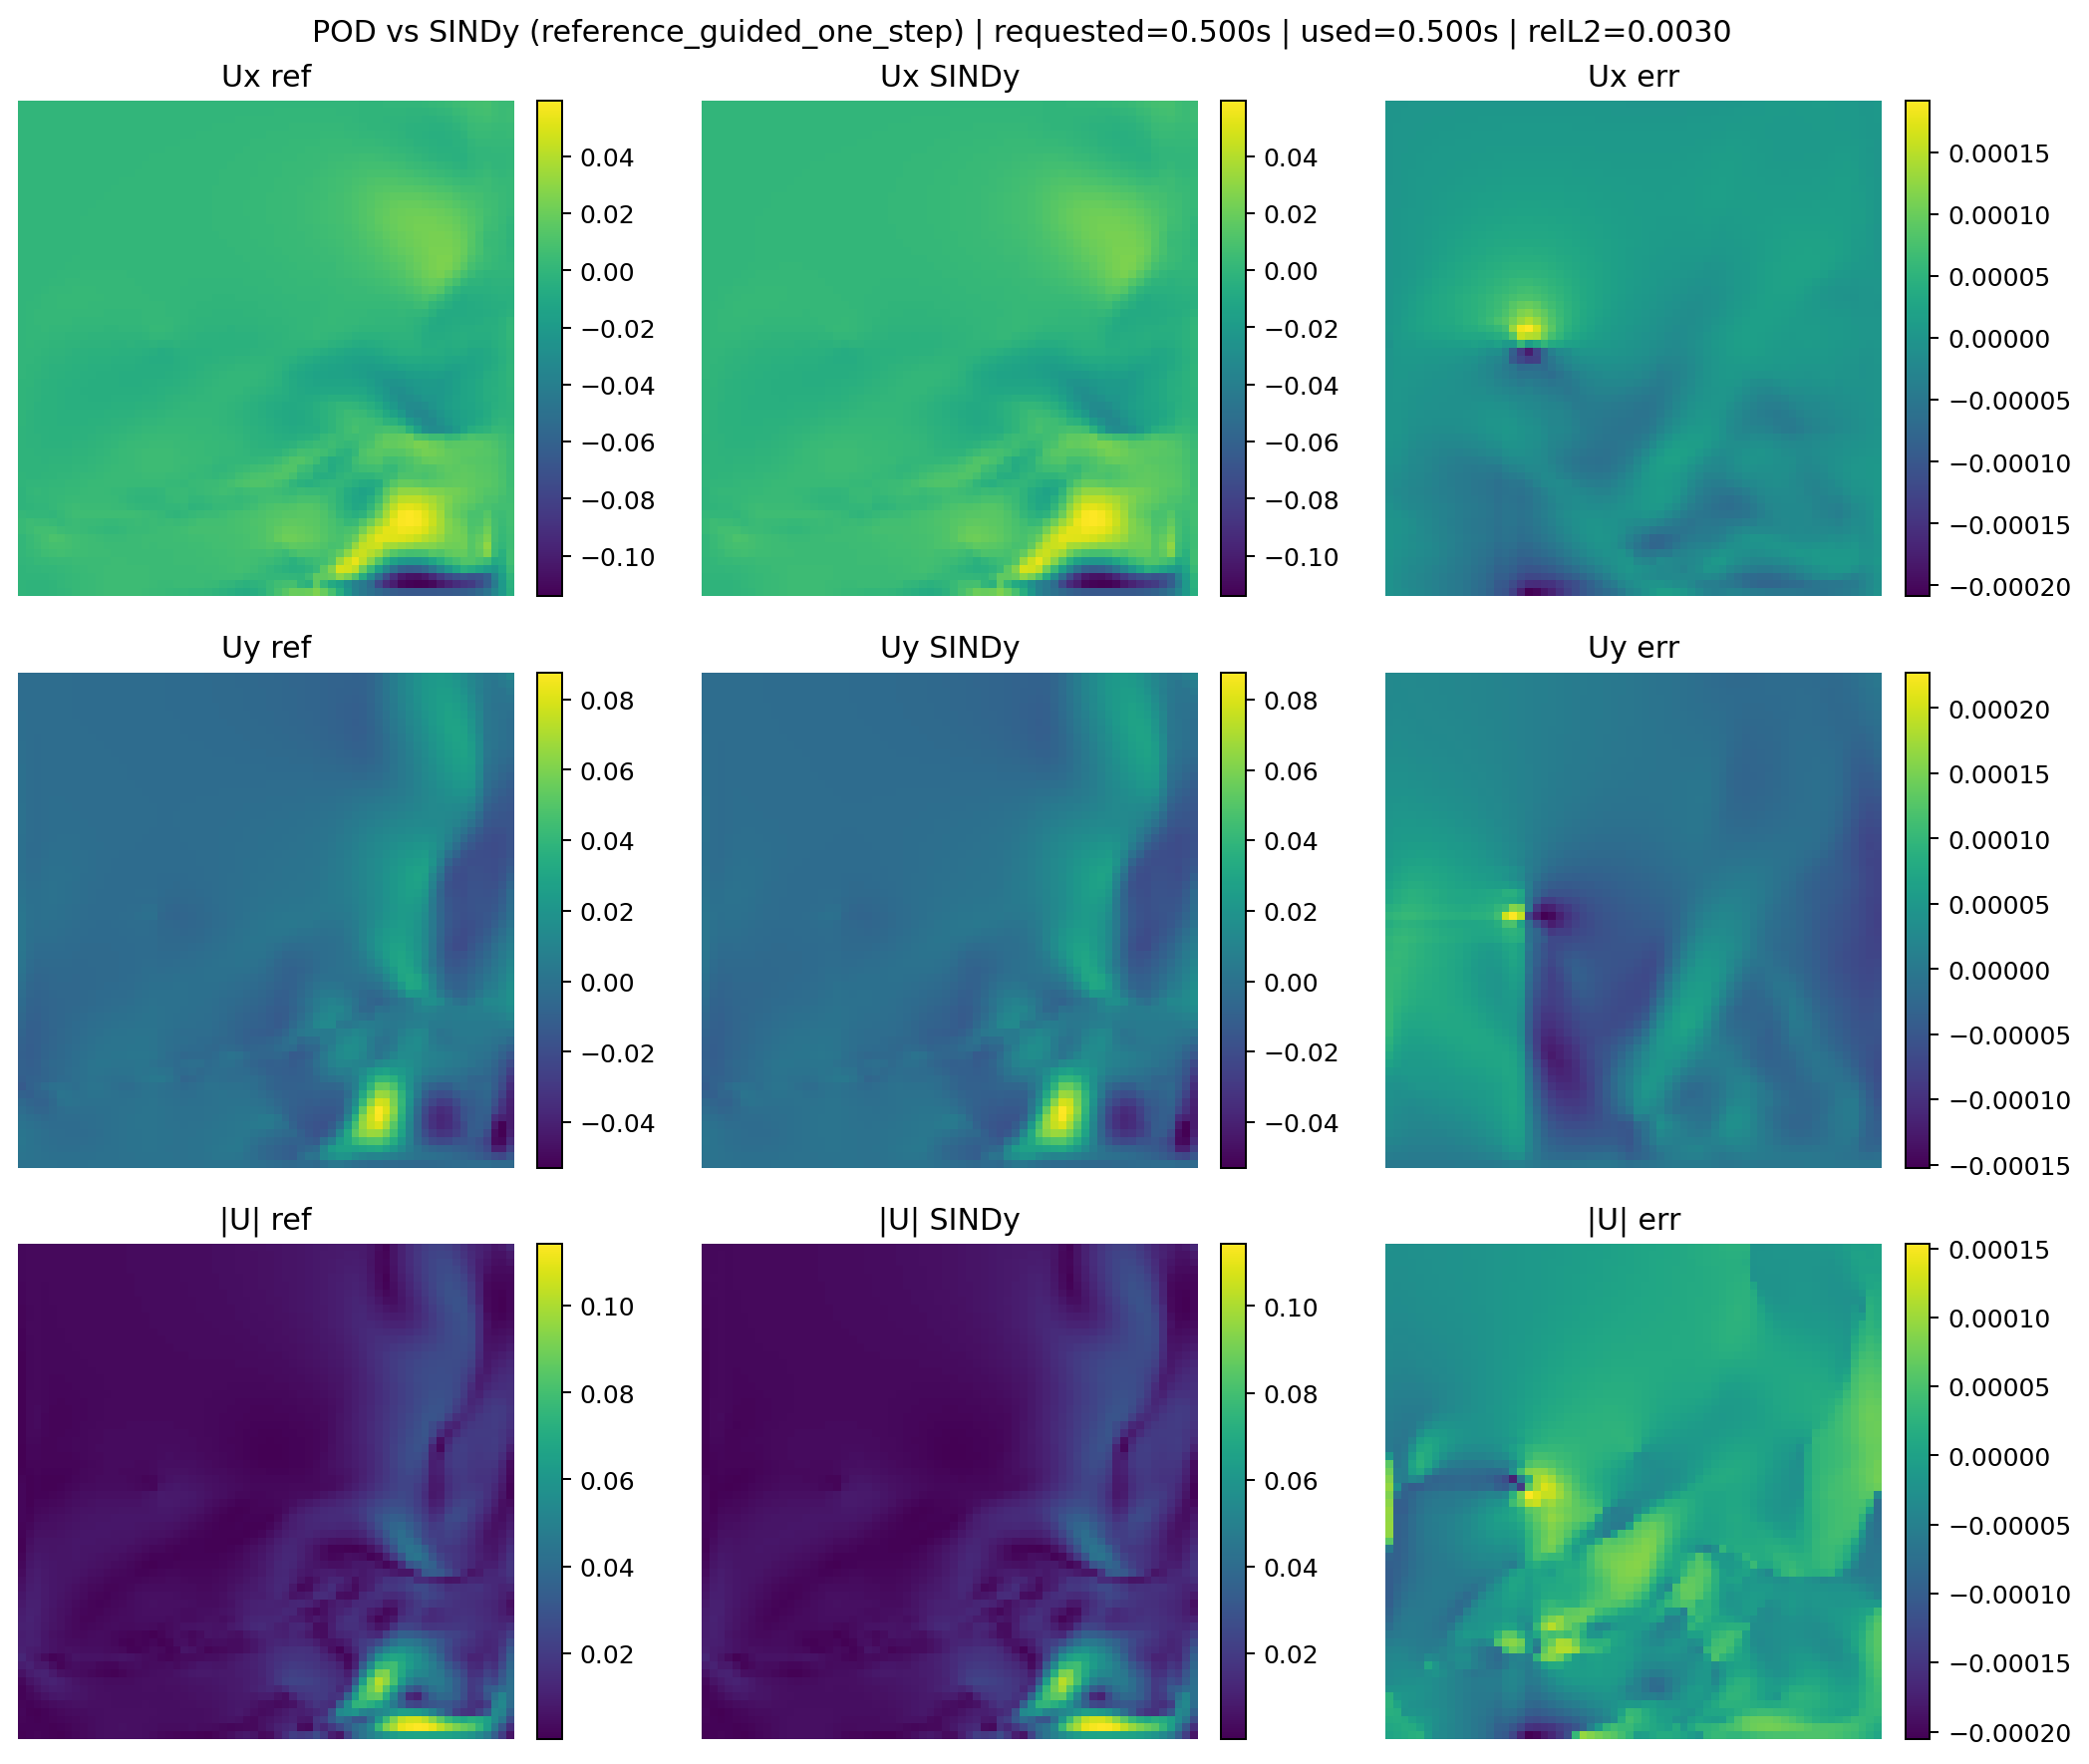
\includegraphics[width=.9\textwidth]{pods_t05.png}\caption{Campo POD--SINDy em $t=\SI{0.5}{s}$.}\end{figure}

A busca de 84 combinações aceitou seis pelo critério baseado em trajetória guiada. O selecionado usa 16 modos, 93,35\% de energia, ordem 2 com senos, $\alpha=3\times10^{-4}$ e 818 termos não nulos em 2960. Apesar do erro guiado 0,00262, a integração livre também falhou. Portanto, ``aceito'' não significa dinamicamente estável.

\subsection{SAE--SINDy}
O modelo usa quatro latentes, ordem 2, seno/cosseno, 23 funções por equação e Lasso com $\alpha=10^{-3}$. Dos 92 coeficientes possíveis, 91 são não nulos: o resultado não é efetivamente esparso. O erro das derivadas é 0,8985; a integração livre falhou e o erro 0,0210 pertence ao método guiado.

\lstinputlisting[style=sindyeq,caption={Equações completas SAE--SINDy.}]{equacoes_sae_sindy.txt}
\begin{figure}[H]\centering
\begin{subfigure}{.49\textwidth}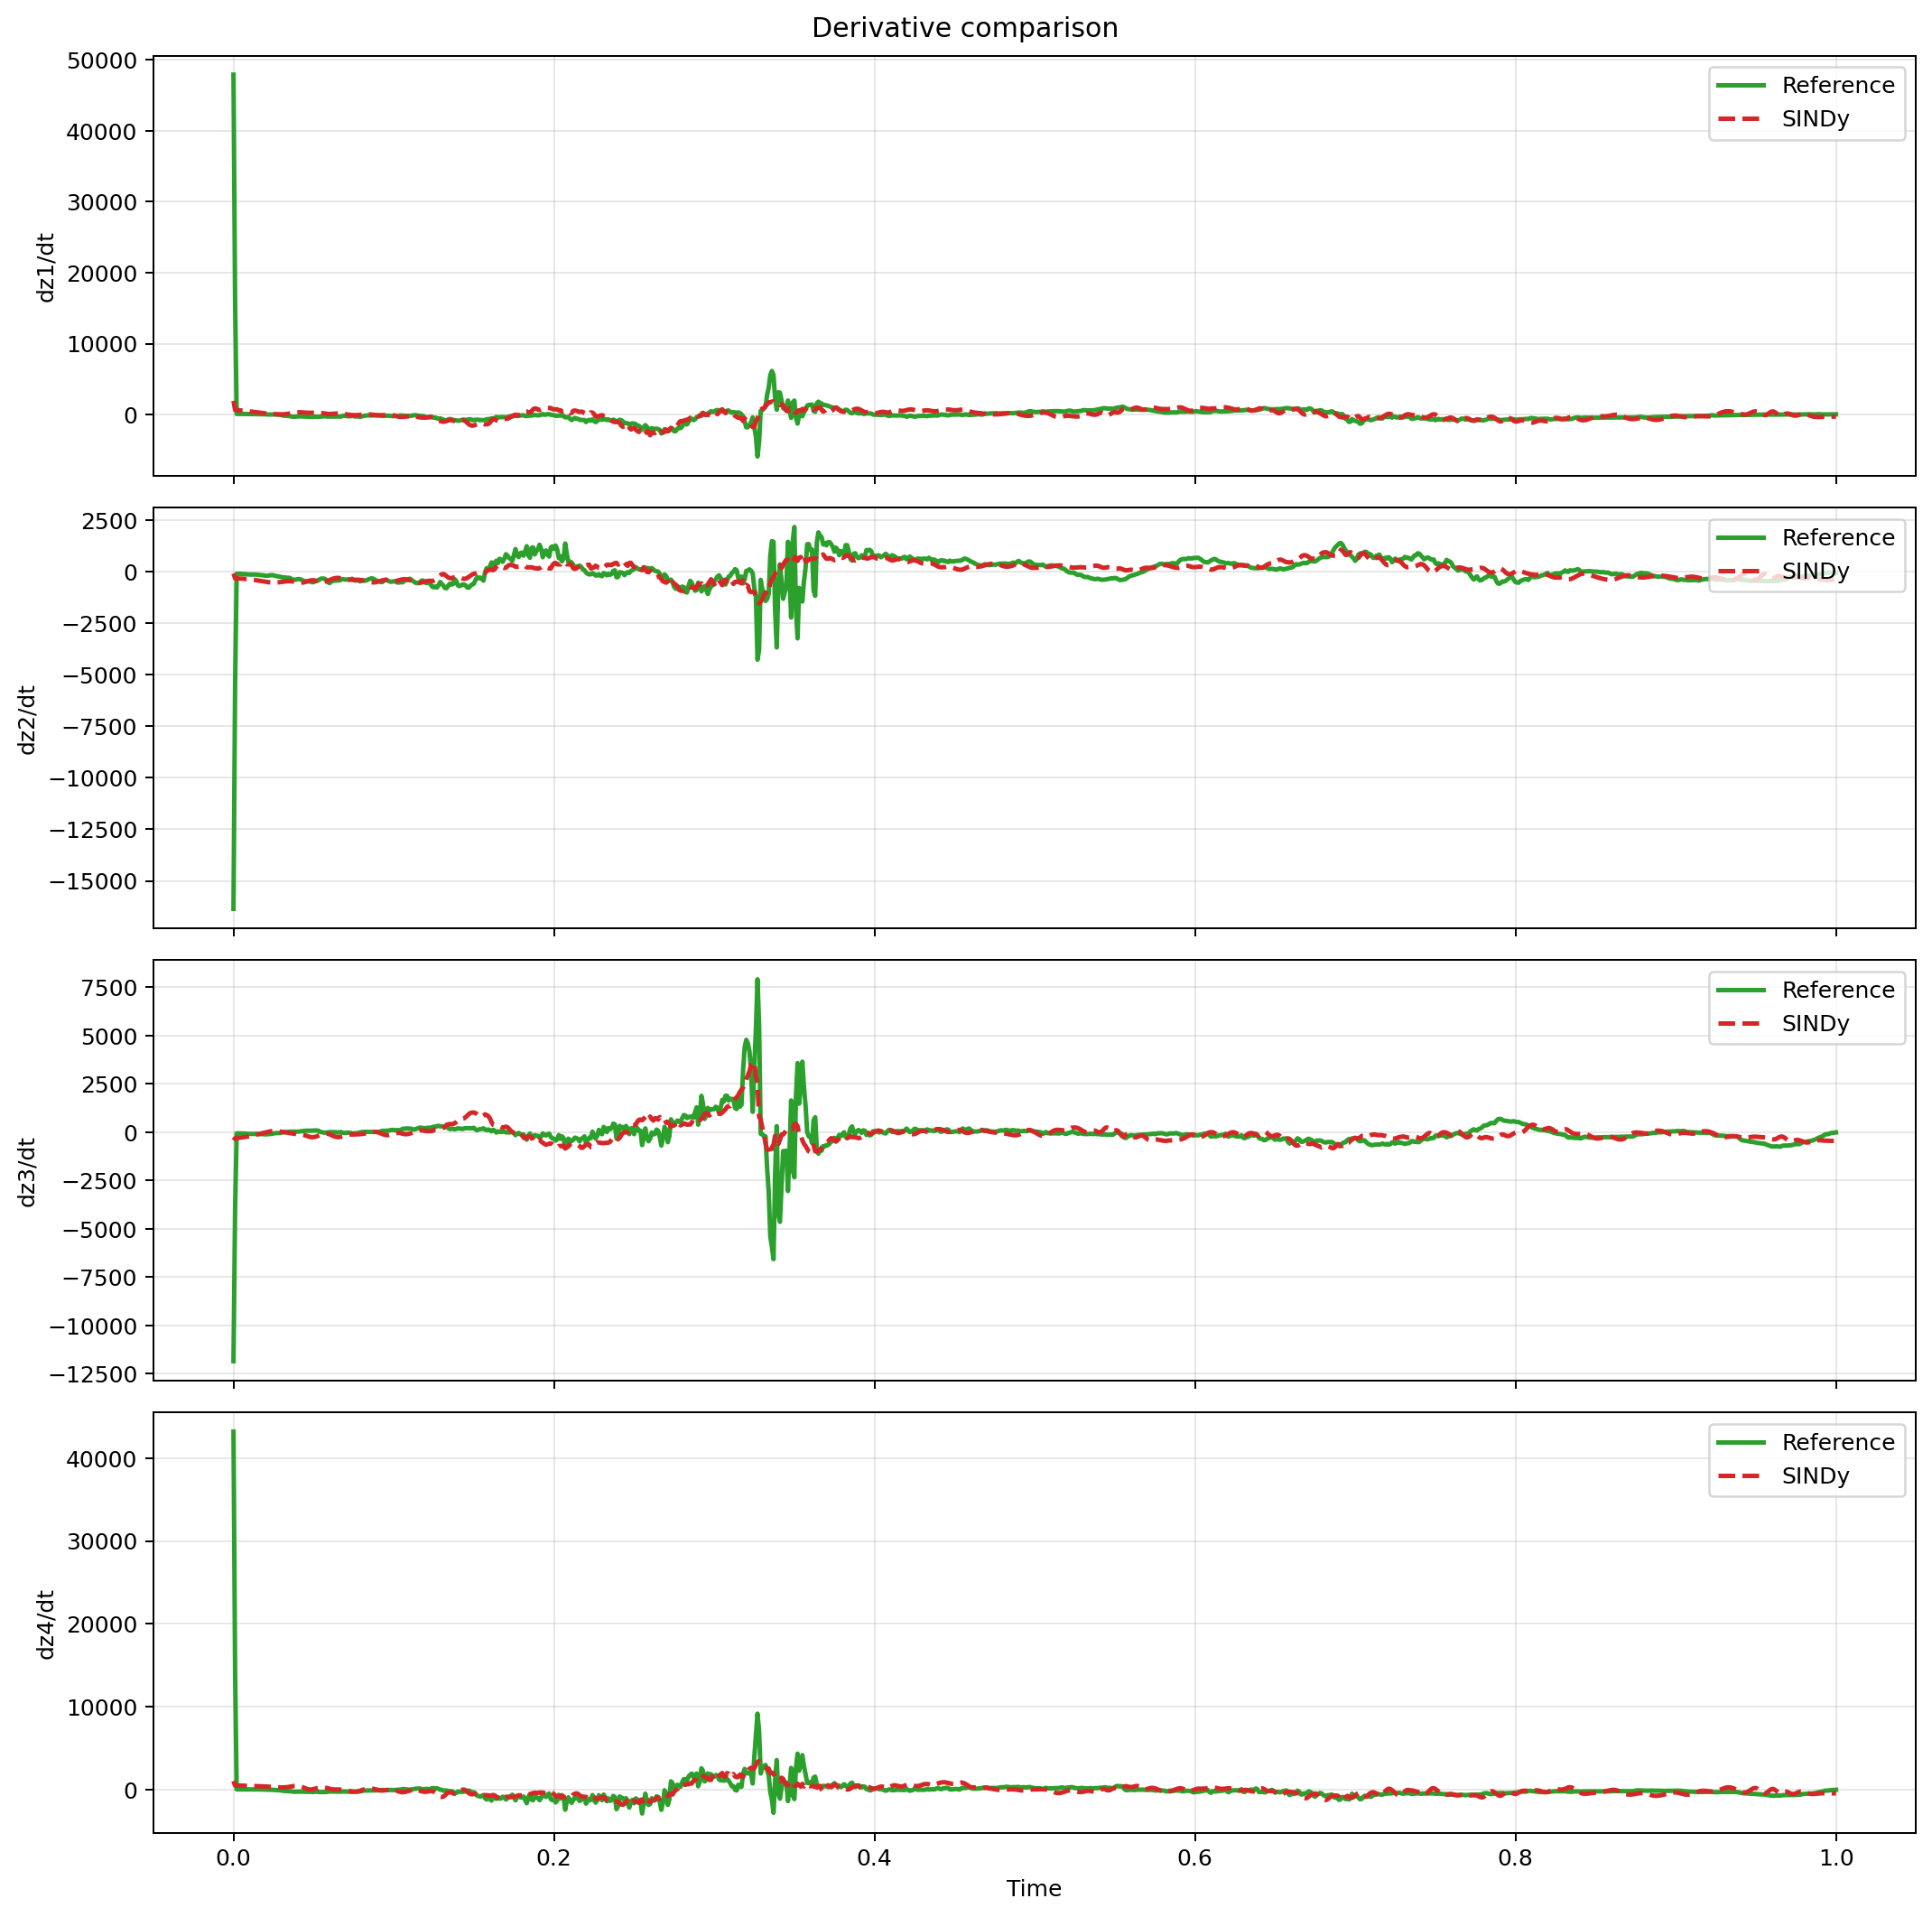
\includegraphics[width=\linewidth]{saes_deriv.png}\caption{Derivadas.}\end{subfigure}
\begin{subfigure}{.49\textwidth}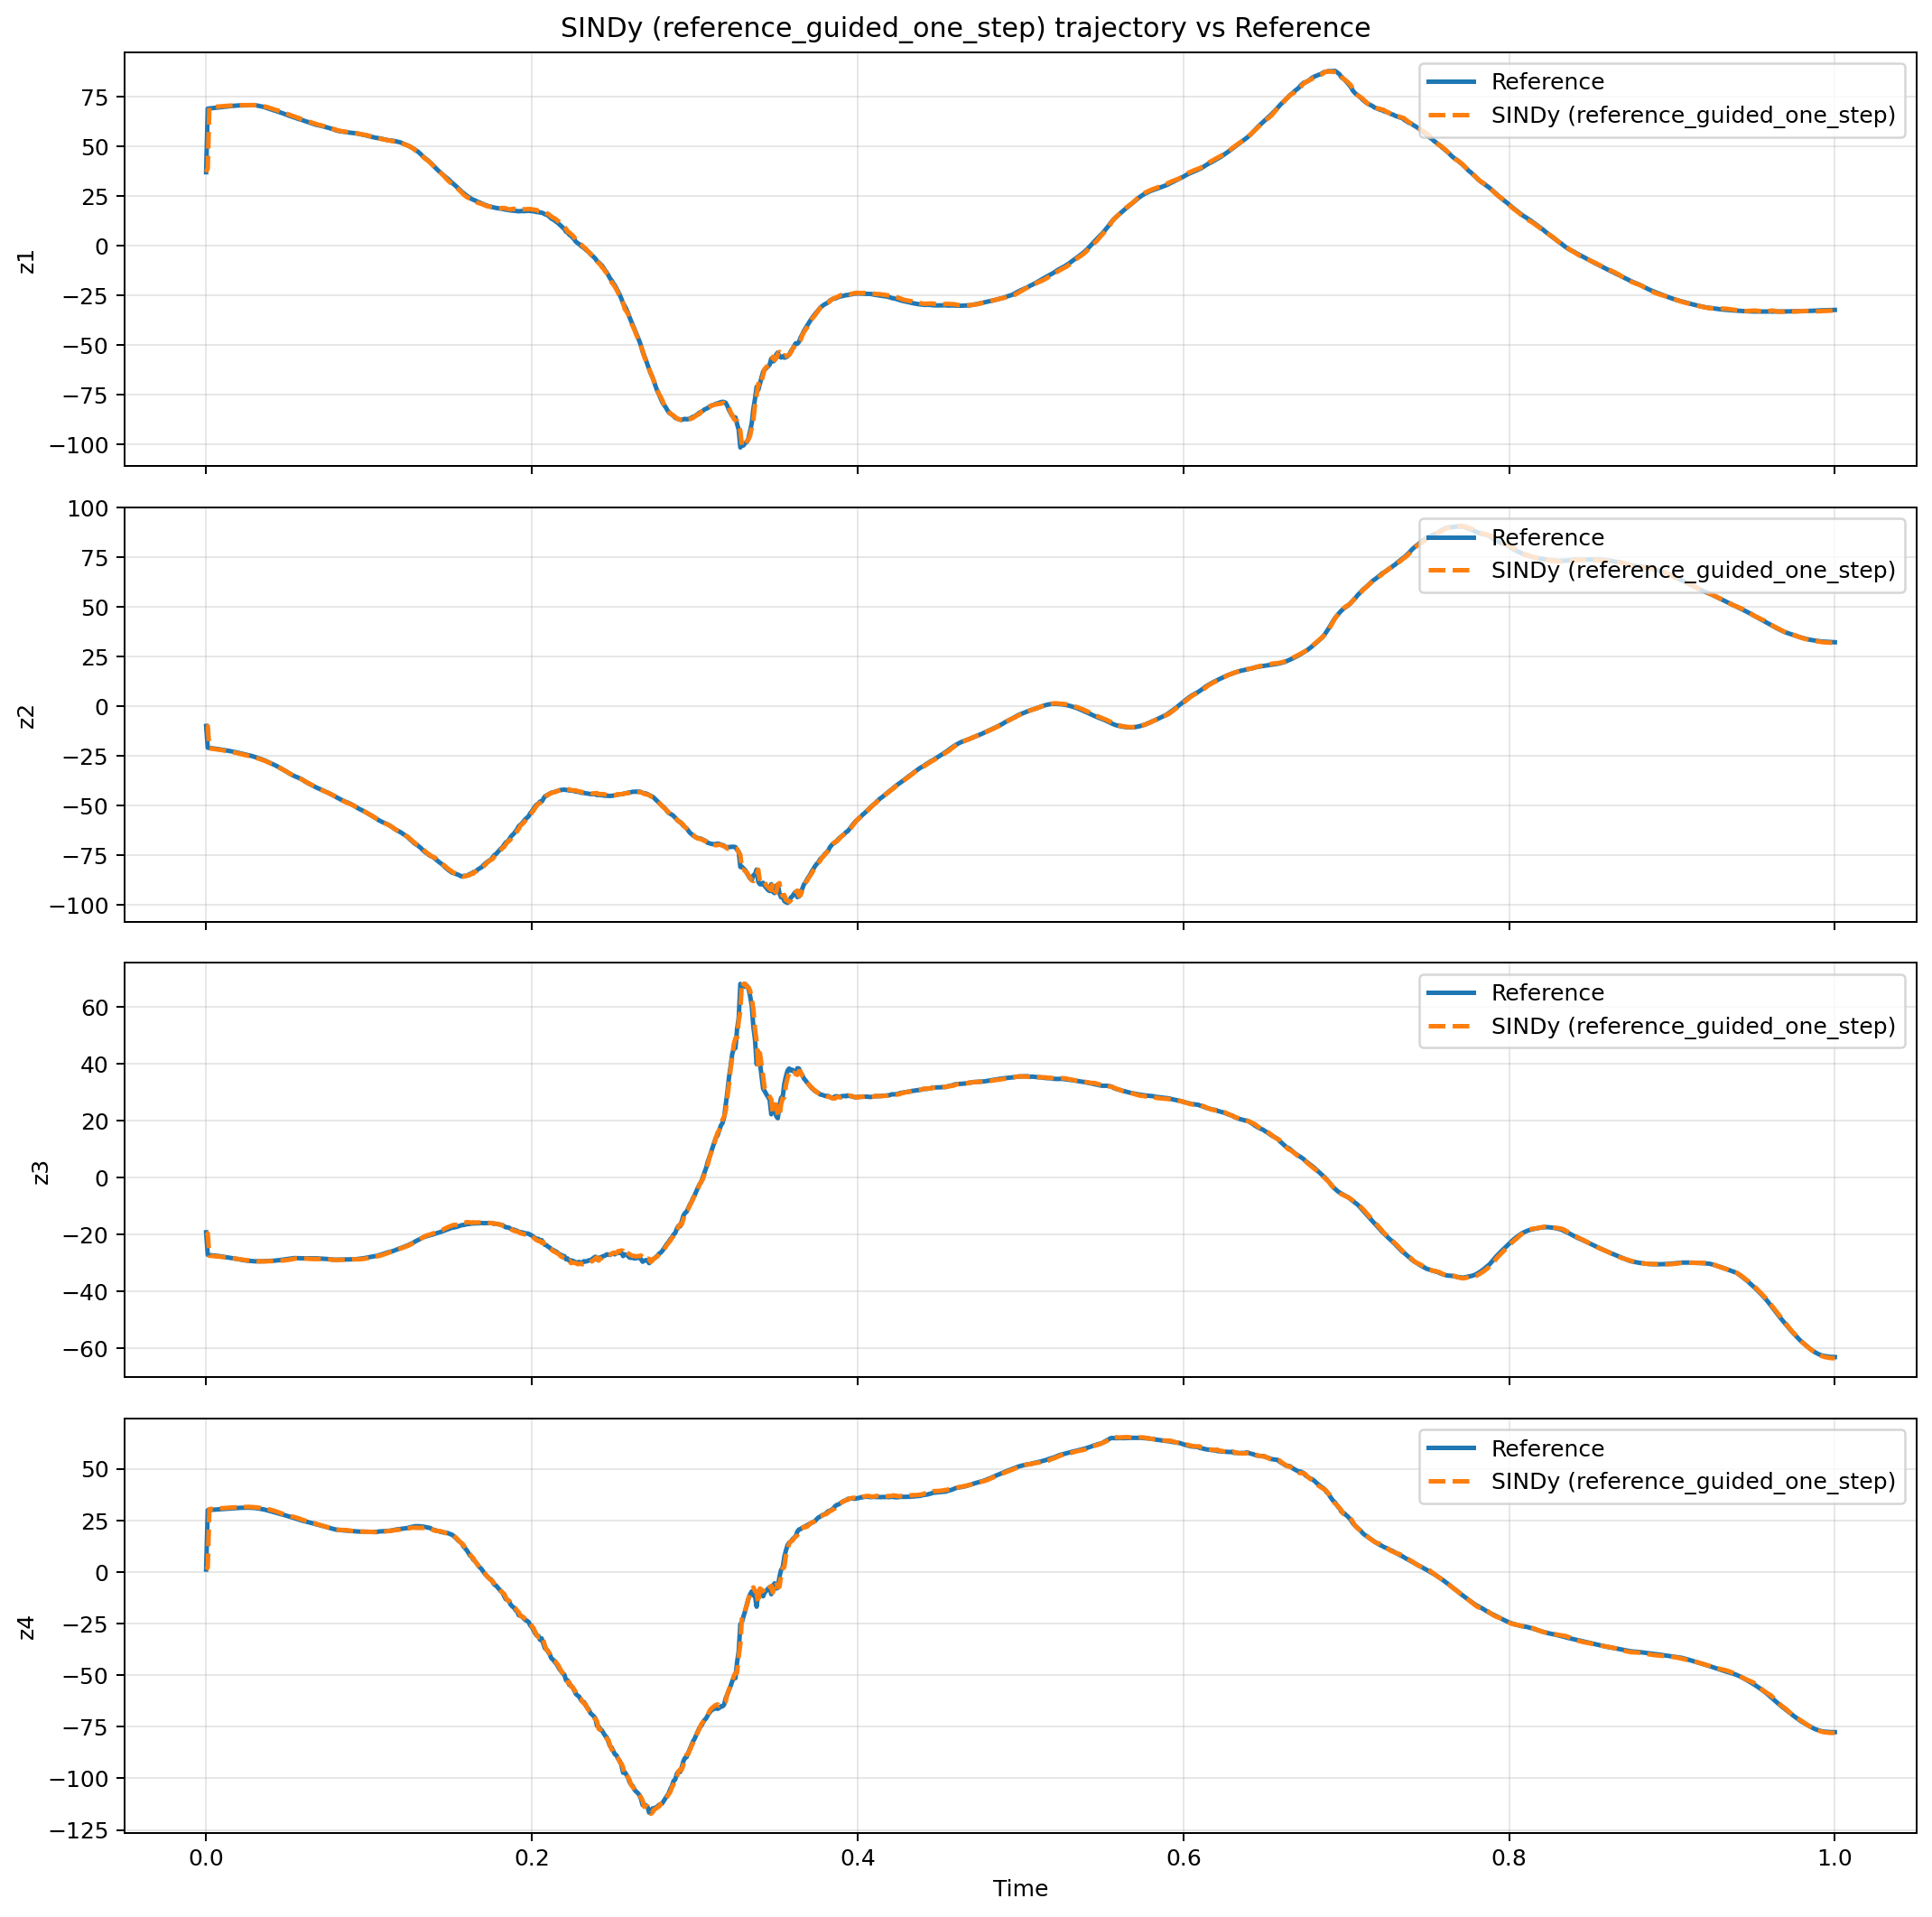
\includegraphics[width=\linewidth]{saes_traj.png}\caption{Trajetória guiada.}\end{subfigure}
\caption{SAE--SINDy: representação local dos dados sem integração autônoma estável.}\end{figure}

\subsection{SAE--POD--SINDy e a POD estabilizadora}
Os quatro latentes foram padronizados e transformados por quatro modos POD. Como a transformação é equidimensional, a energia preservada é numericamente 100\%, alinhando-se à estratégia de Lin, Xiao e Fang~\cite{lin2024}: a POD centraliza e ortogonaliza os códigos do SAE sem compressão adicional, buscando uma variedade mais suave para regressão.

O melhor modelo entre 48 candidatos---40 aceitos---usa ordem 1, Lasso adaptativo, $\alpha=0,01$, janela Savitzky--Golay 21, termos polinomiais em tempo, sem senos e RK45. A biblioteca tem oito termos por equação e 27 coeficientes não nulos em 32.

\begin{table}[H]\centering
\caption{Resultados SAE--POD--SINDy.}\label{tab:hyb}
\begin{tabular}{lr}\toprule Métrica & Valor\\\midrule
Energia POD latente&1,0000\\Erro de derivada / $R^2$&0,9026 / 0,1850\\Erro de um passo / $R^2$&0,03008 / 0,99910\\Integração livre&bem-sucedida\\Erro livre / $R^2$&0,55091 / 0,69650\\\bottomrule\end{tabular}\end{table}

\lstinputlisting[style=sindyeq,caption={Equações completas SAE--POD--SINDy.}]{equacoes_sae_pod_sindy.txt}
\begin{figure}[H]\centering
\begin{subfigure}{.49\textwidth}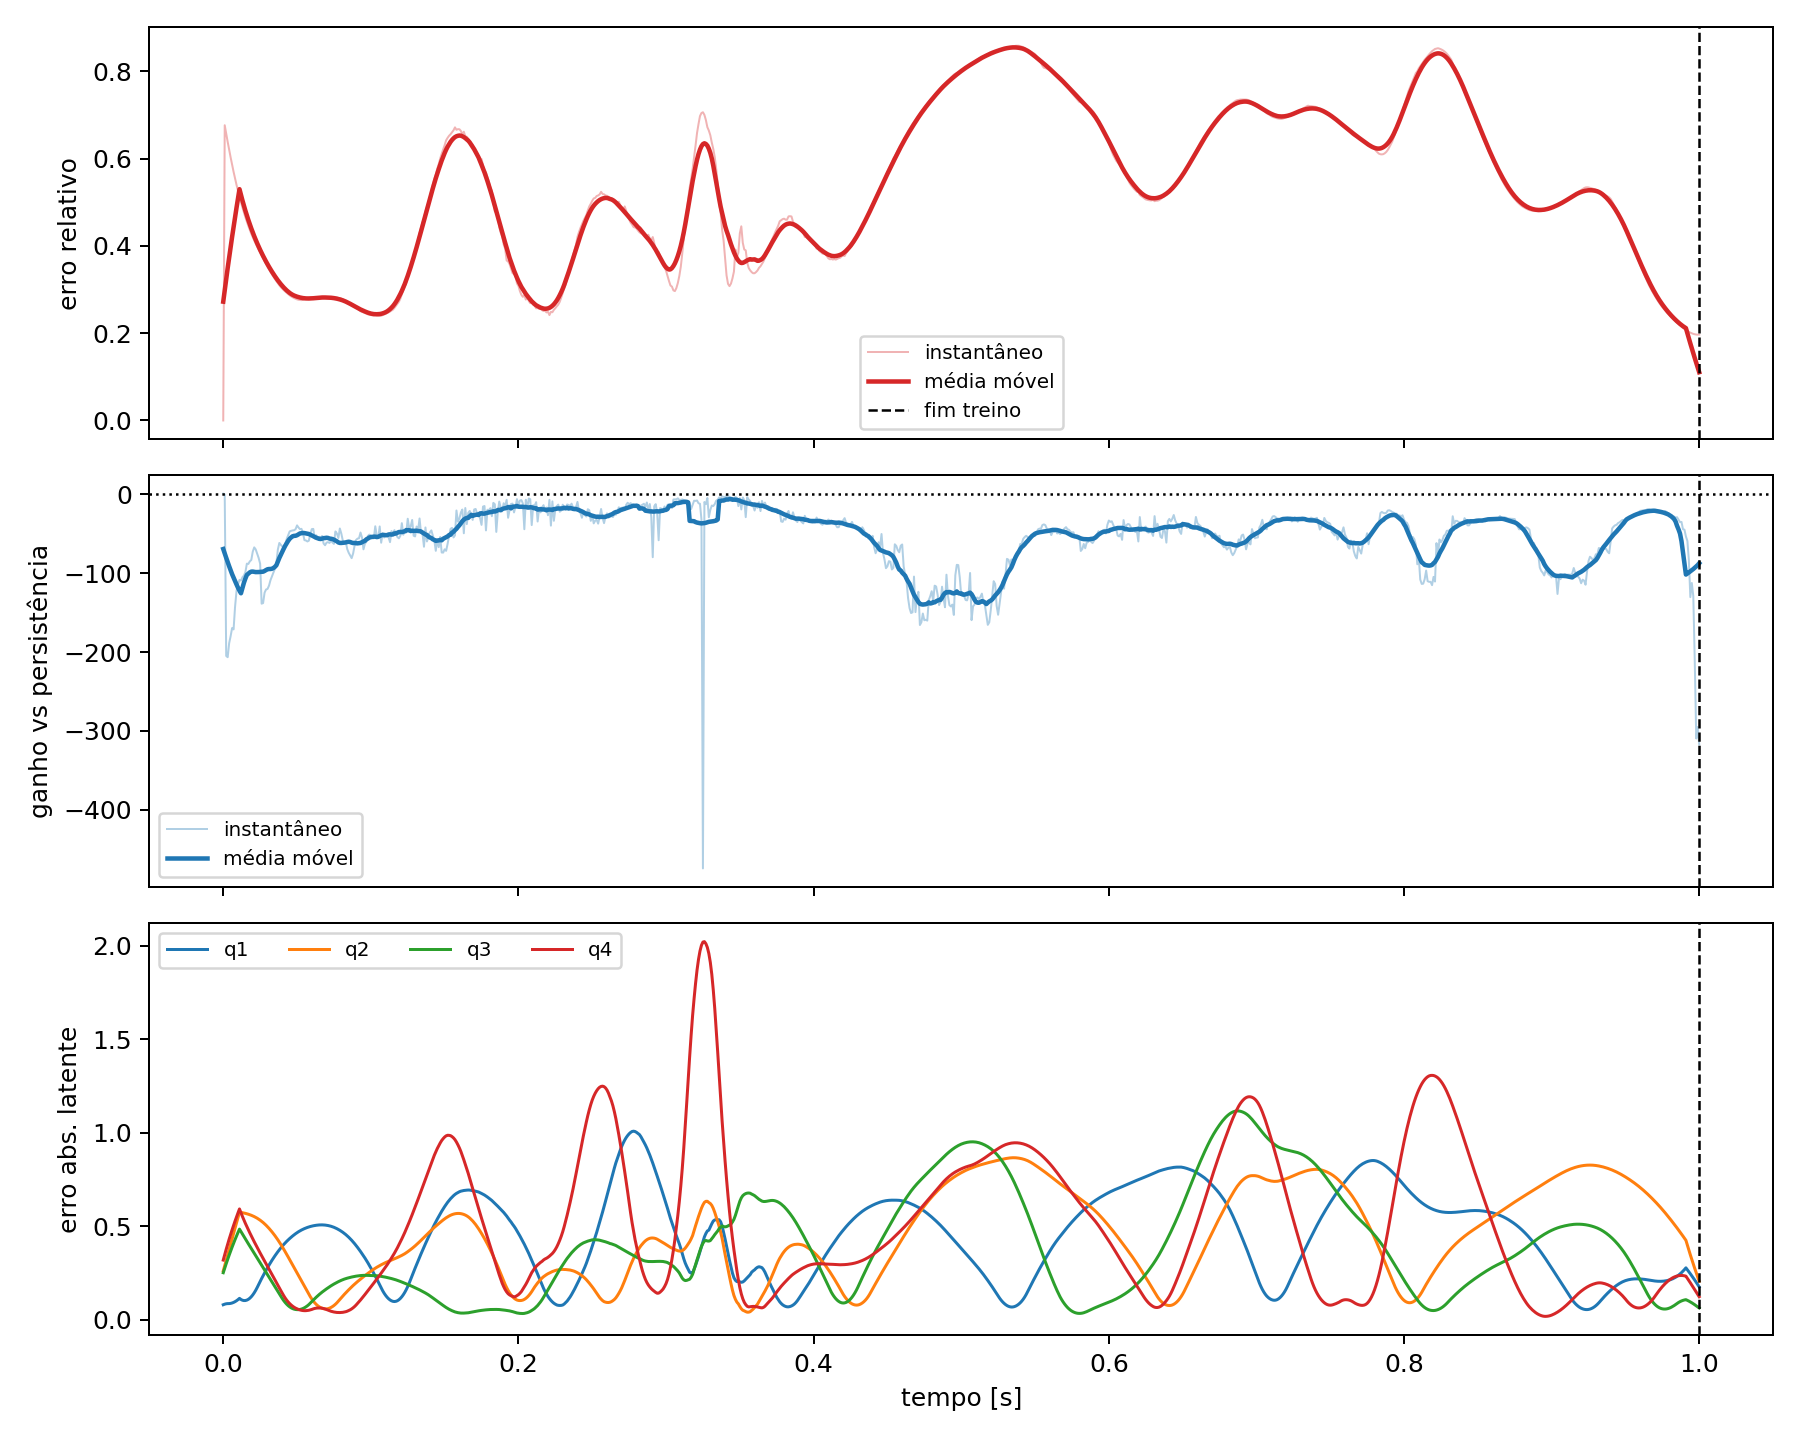
\includegraphics[width=\linewidth]{hyb_curves.png}\caption{Erro temporal.}\end{subfigure}
\begin{subfigure}{.49\textwidth}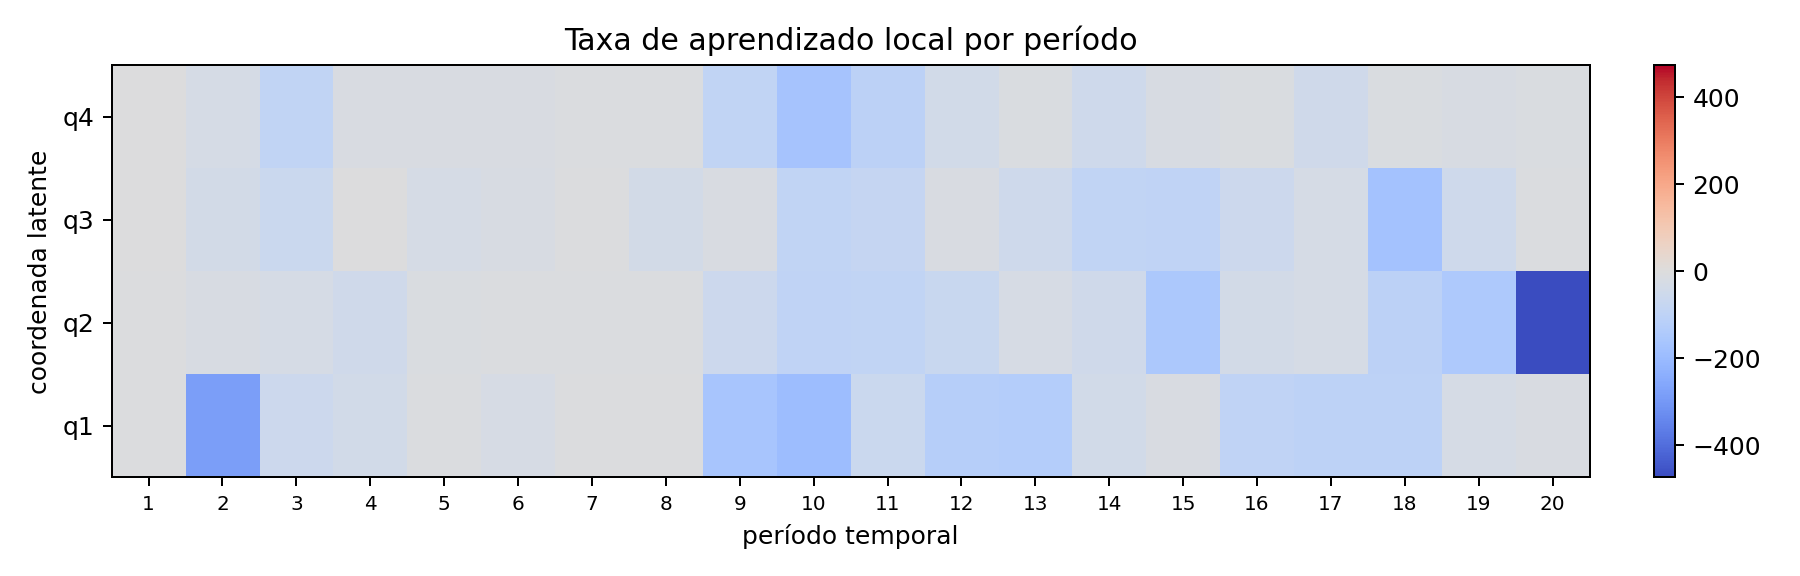
\includegraphics[width=\linewidth]{hyb_map.png}\caption{Mapa das coordenadas.}\end{subfigure}
\caption{Diagnóstico temporal do modelo estabilizado.}\end{figure}
\begin{figure}[H]\centering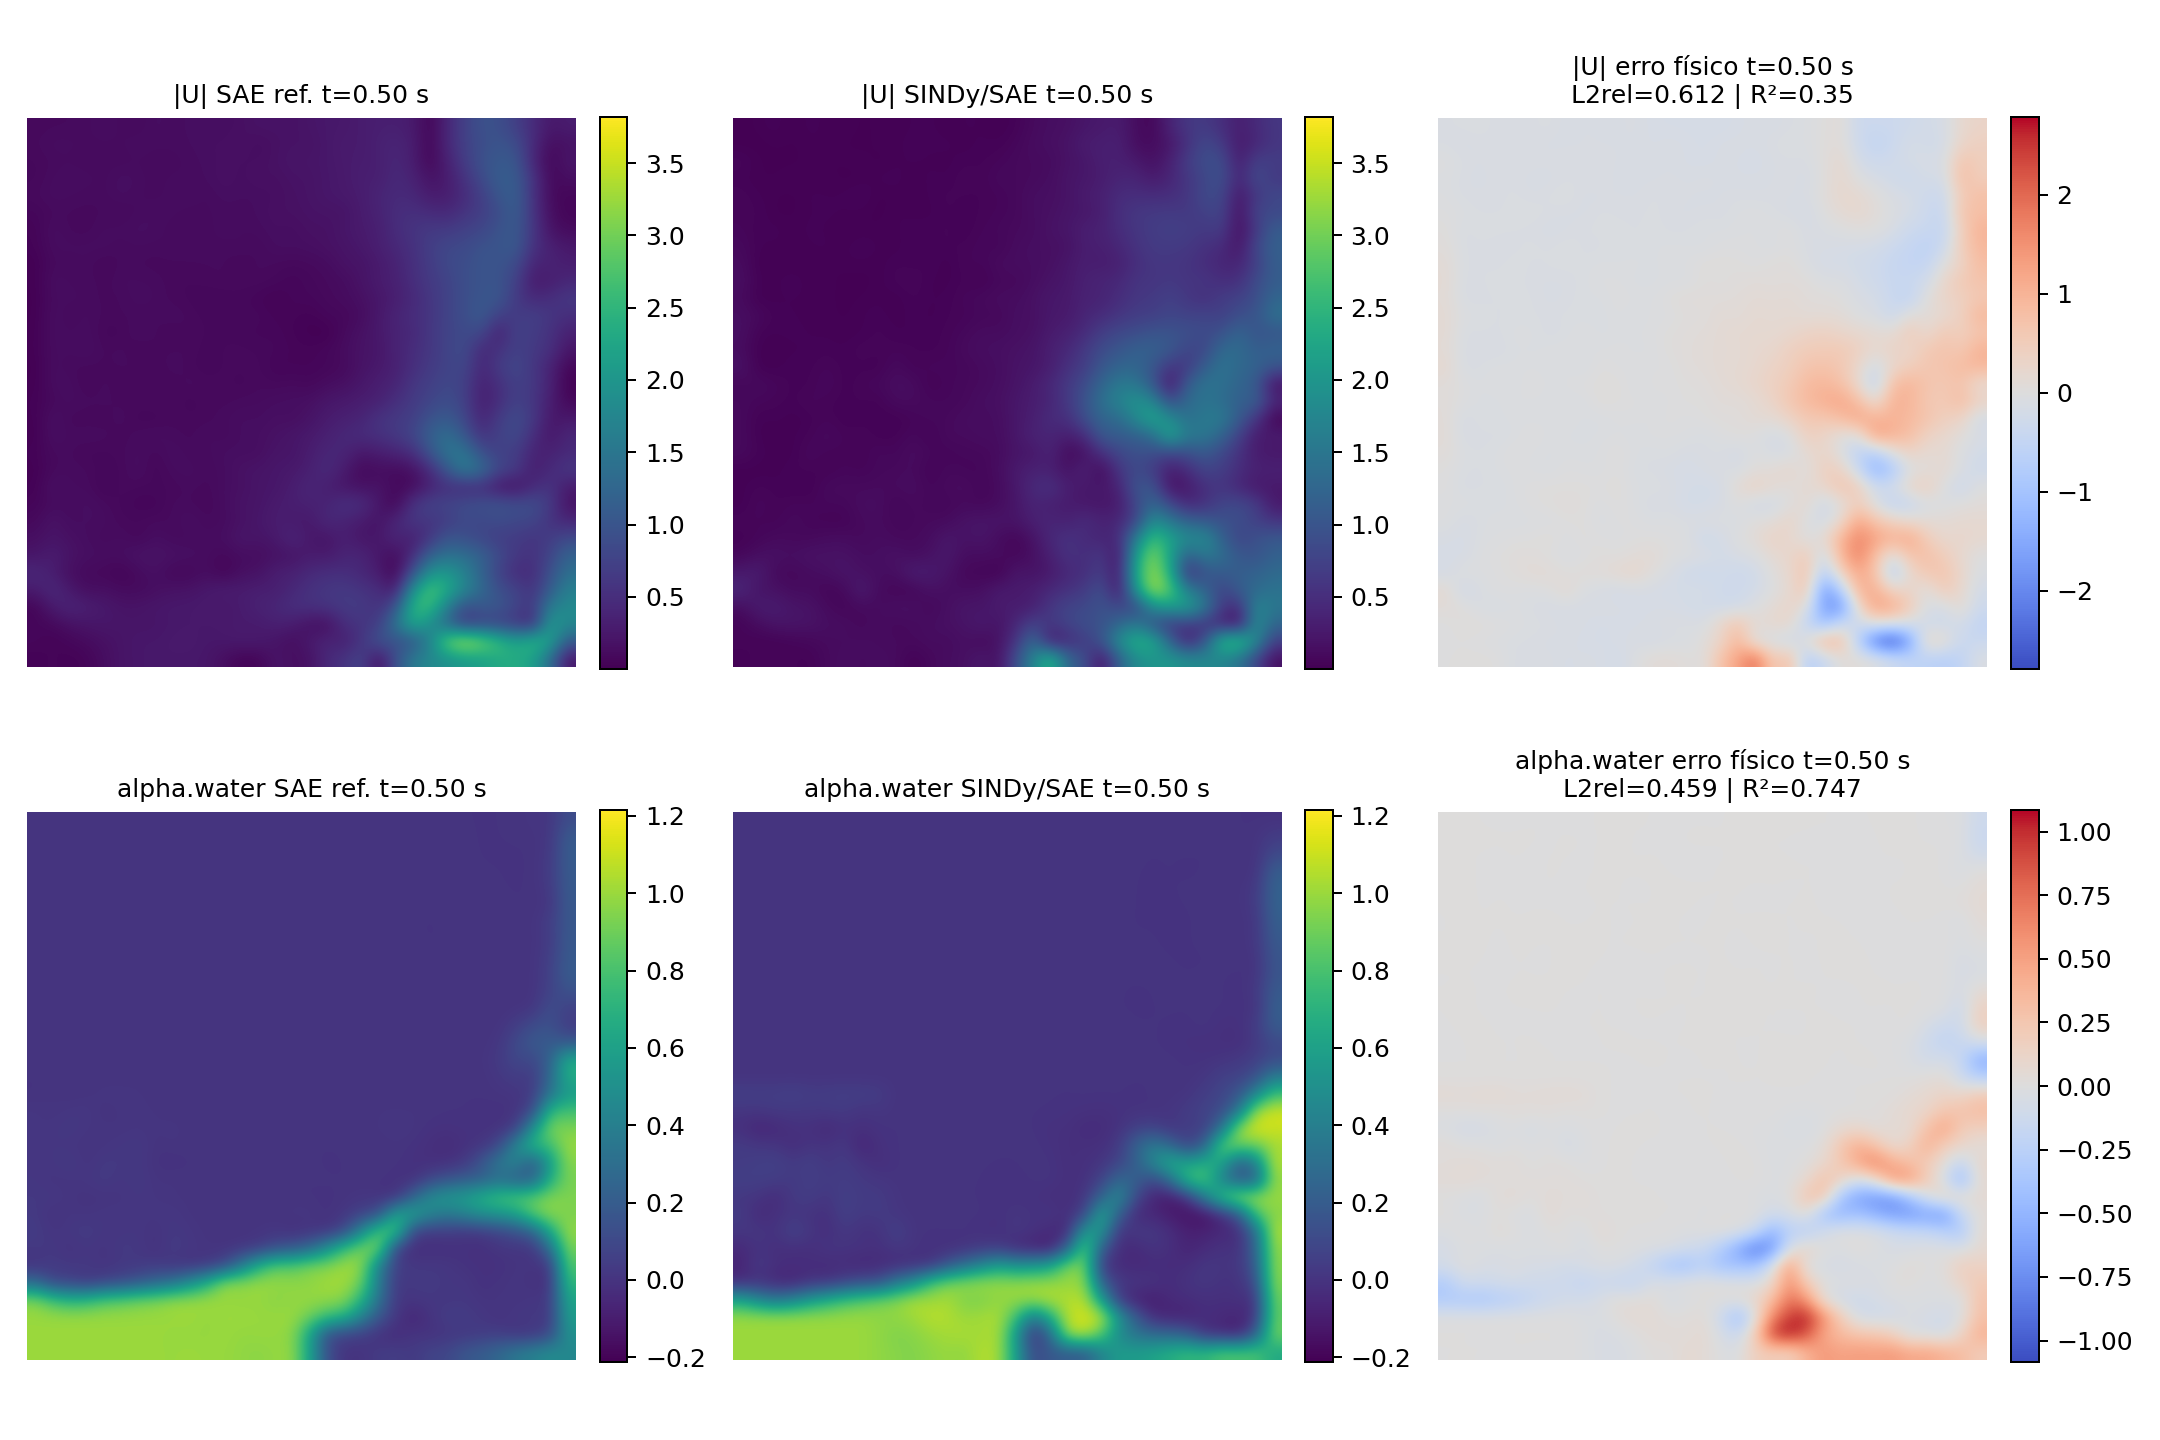
\includegraphics[width=.91\textwidth]{hyb_t05.png}\caption{Campos decodificados da integração livre em $t=\SI{0.5}{s}$.}\end{figure}
\begin{figure}[H]\centering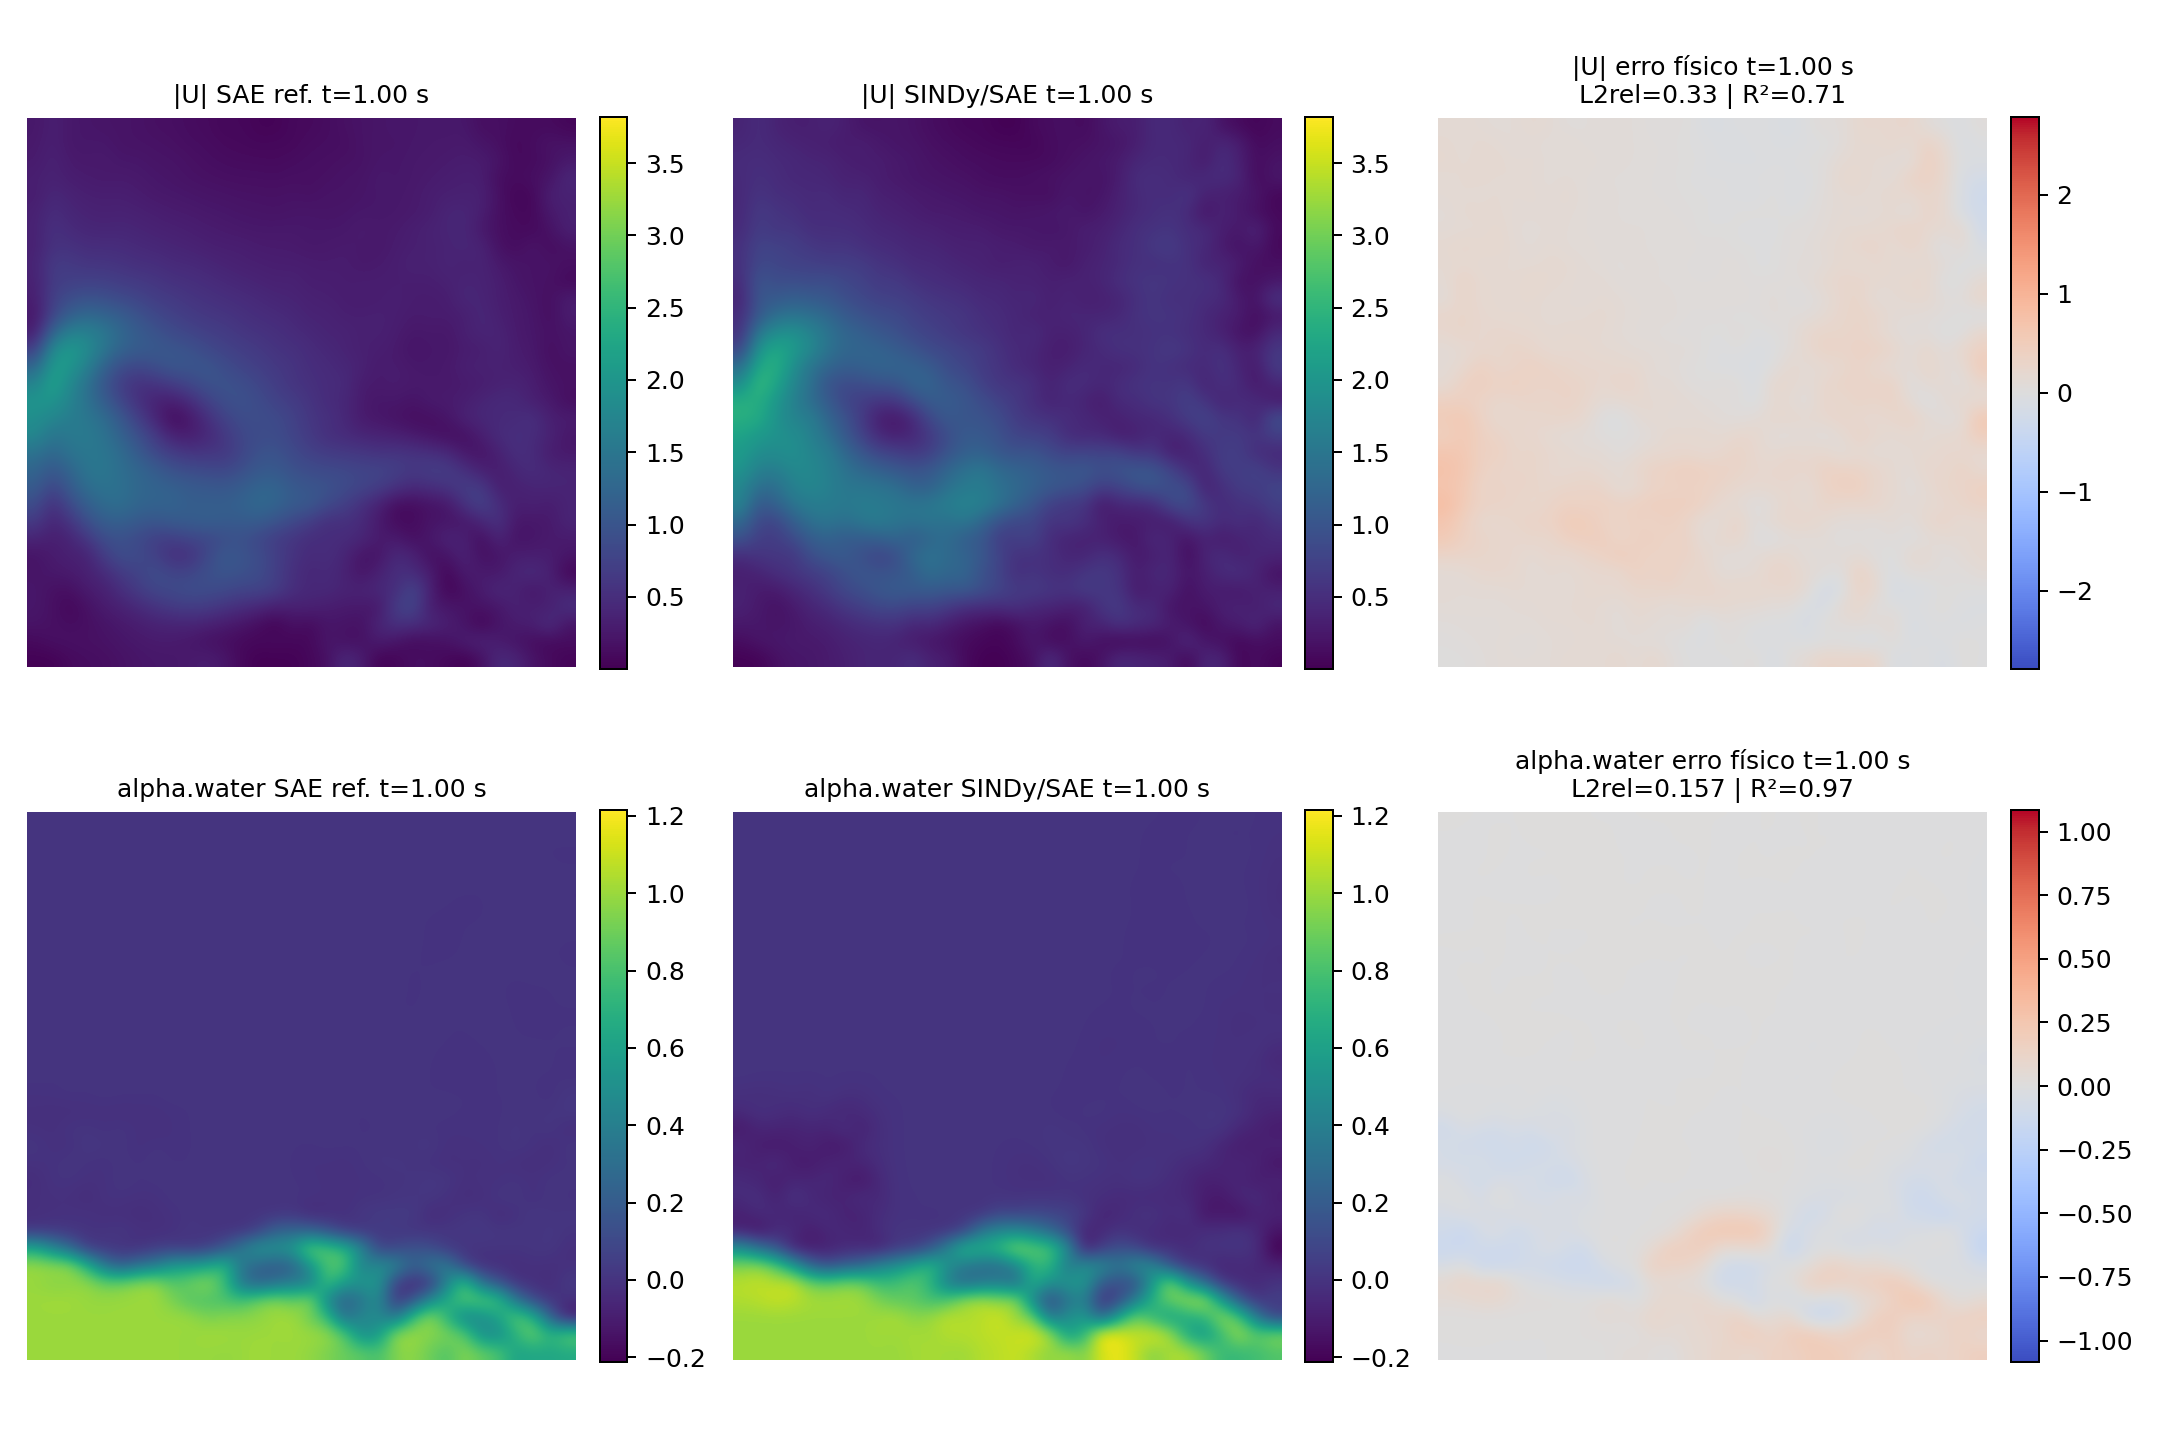
\includegraphics[width=.91\textwidth]{hyb_t10.png}\caption{Campos decodificados em $t=\SI{1}{s}$.}\end{figure}

Nas comparações decodificadas, em $t=0,25;0,50;0,75;1,00\,\si{s}$, o erro de $|U|$ é, respectivamente, 0,289; 0,612; 0,376; 0,330, e o erro de $\alpha_{water}$ é 0,214; 0,459; 0,238; 0,157. A interface é mais robusta que a velocidade. O relatório direto com OpenFOAM tem divisão por norma quase zero em $t=0$, gerando número gigantesco; esse ponto não deve ser interpretado fisicamente.

\section{Relação com Lin, Xiao e Fang}
Lin, Xiao e Fang~\cite{lin2024} propõem exatamente a sequência conceitual usada aqui: SAE para variedade não linear, POD para estabilizar os códigos e SINDy para descobrir equações. Os autores atribuem a instabilidade latente à aleatoriedade do SAE e argumentam que a POD melhora centralização, ortogonalidade e suavidade, facilitando aproximações polinomiais esparsas. Em seus casos de lock exchange e cilindros, SAE--POD--SINDy supera SAE--SINDy em correlação e RMSE.

O caso URANS fornece evidência qualitativamente coerente: SAE--SINDy puro falha na integração, enquanto a transformação POD equidimensional preserva toda a energia e permite integrar até $t=1\,\si{s}$. Esse é um ganho claro de estabilidade. Porém, a derivada continua mal ajustada ($R^2=0,185$) e o erro livre é 0,551; portanto, não se deve concluir que a POD resolveu completamente a descoberta dinâmica.

\begin{table}[H]\centering
\caption{Representação de dados versus dinâmica.}\label{tab:repdyn}
\begin{tabularx}{\textwidth}{>{\bfseries}l X X}
\toprule Caso & O que representa & Conclusão\\\midrule
POD isolada & snapshots de velocidade em base linear & sem lei temporal\\
SAE isolado & cinco campos em variedade não linear & sem lei temporal\\
POD--SINDy & dinâmica das amplitudes POD & somente ajuste guiado; livre falha\\
SAE--SINDy & dinâmica dos latentes & quase denso; livre falha\\
SAE--POD--SINDy & dinâmica dos códigos ortogonalizados & livre funciona, mas com erro 0,551\\
\bottomrule\end{tabularx}\end{table}

Logo, os casos isolados POD e SAE são puramente representacionais. Os casos com SINDy tentam representar dinâmica; contudo, POD--SINDy e SAE--SINDy tiveram sucesso apenas local. A POD estabilizadora também não cria dinâmica---quem a cria é o SINDy---mas oferece coordenadas nas quais a integração se tornou possível.

\section{Pontos positivos, negativos e recomendações}
\subsection*{Positivos}
\begin{itemize}
\item 10001 saídas CFD fornecem excelente resolução temporal para diferenciação;
\item POD: 99,36\% de energia e erro global 8,02\% com 50 modos;
\item SAE: $R^2$ de 0,949/0,942 em treino/validação e latente de dimensão quatro;
\item POD latente equidimensional preserva 100\% da energia;
\item somente o SAE--POD--SINDy completa integração livre, com $R^2=0,697$;
\item 40 de 48 candidatos híbridos atenderam aos limites definidos.
\end{itemize}
\subsection*{Negativos}
\begin{itemize}
\item Euler de primeira ordem, uma célula em $z$ e ausência de verificação de malha/passo;
\item notebook e artefatos SAE/POD não estão sincronizados;
\item POD--SINDy e SAE--SINDy falham em integração livre;
\item o SAE--SINDy mantém 91 de 92 coeficientes e não é parcimonioso;
\item o modelo híbrido tem baixo ajuste de derivadas e erro livre ainda elevado;
\item os rótulos treino/validação do diagnóstico híbrido não são confiáveis: após ordenar tempos, o código usa um corte de 801 amostras, mas os NPZ indicam que ambos os conjuntos originais cobrem quase todo o intervalo;
\item termos explícitos em $t$ tornam o modelo híbrido não autônomo e podem ajustar a realização específica em vez de uma lei geral.
\end{itemize}

\subsection*{Recomendações}
\begin{enumerate}
\item Versionar notebook, modelo, normalizador, latentes e configuração em um único manifesto; não sobrescrever artefatos.
\item Reexecutar SAE puro e SAE--POD com a mesma divisão temporal e comparar POD equidimensional versus truncada.
\item Selecionar SINDy pelo erro livre em validação temporal, nunca pelo erro guiado.
\item Normalizar a biblioteca, testar Adalasso/STLSQ/SR3 e derivadas regularizadas.
\item Penalizar dinâmica no treino do SAE para que os latentes sejam suaves e previsíveis.
\item Avaliar conservação de massa, limites de $\alpha$, energia cinética e campos $k,\omega$.
\item Fazer estudos de malha, passo e modelo de turbulência; comparar URANS com LES e dados de referência.
\end{enumerate}

\section{Conclusão}
A POD e o SAE representam os dados com boa precisão, mas isoladamente não modelam evolução. Nos dois SINDy sem estabilizador, as métricas guiadas são pequenas, porém a integração livre falha; logo, os resultados são predominantemente locais. A POD aplicada aos quatro latentes segue diretamente a motivação de Lin, Xiao e Fang: condiciona o espaço sem perda de energia e torna possível a integração autônoma. O ganho é mais claro neste URANS do que no caso LES previamente analisado, mas o erro livre 0,551 impede classificar o modelo como plenamente validado. O resultado sustenta a necessidade prática do estabilizador para este conjunto de latentes, não a suficiência da POD para garantir dinâmica correta.

\appendix
\section{Arquivos principais}
\small
\begin{itemize}
\item OpenFOAM: \path{system/controlDict}, \path{system/fvSchemes}, \path{system/fvSolution}, \path{system/blockMeshDict}, \path{constant/momentumTransport}.
\item POD: \path{POD/resultados/resultados_pod_completos.npz}.
\item SAE: \path{SAE/resultados/sae_dense.keras}, \path{sae_dense_metrics.npz}, \path{latents.npz}.
\item SINDy: JSON, CSV, NPZ e equações em \path{SINDy/resultados}.
\end{itemize}\normalsize

\begin{thebibliography}{9}
\bibitem{nicoud} F. R. Menter. Two-equation eddy-viscosity turbulence models for engineering applications. \emph{AIAA Journal}, 32, 1994.
\bibitem{sirovich} L. Sirovich. Turbulence and the dynamics of coherent structures. \emph{Quarterly of Applied Mathematics}, 45, 1987.
\bibitem{hinton} G. E. Hinton e R. R. Salakhutdinov. Reducing the dimensionality of data with neural networks. \emph{Science}, 313, 2006.
\bibitem{brunton} S. L. Brunton, J. L. Proctor e J. N. Kutz. Discovering governing equations from data by sparse identification of nonlinear dynamical systems. \emph{PNAS}, 113, 2016.
\bibitem{lin2024} X. Lin, D. Xiao e F. Fang. Data discovery of low dimensional fluid dynamics of turbulent flows. \emph{arXiv:2401.05449}, 2024. \href{https://arxiv.org/abs/2401.05449}{arxiv.org/abs/2401.05449}.
\bibitem{openfoam} OpenFOAM Foundation. \emph{OpenFOAM 13 documentation}.
\end{thebibliography}
\end{document}
